%% For double-blind review submission
%%\documentclass[acmsmall,anonymous,review]{acmart}\settopmatter{printfolios=true}
%% For single-blind review submission
%\documentclass[acmsmall,review]{acmart}\settopmatter{printfolios=true}
%% For final camera-ready submission
\documentclass[acmsmall,screen]{acmart}\settopmatter{}
\citestyle{acmauthoryear}

%% Note: Authors migrating a paper from PACMPL format to traditional
%% SIGPLAN proceedings format should change 'acmlarge' to
%% 'sigplan,10pt'.


%% Some recommended packages.
\usepackage{booktabs}   %% For formal tables:
                        %% http://ctan.org/pkg/booktabs
\usepackage{subcaption} %% For complex figures with subfigures/subcaptions
                        %% http://ctan.org/pkg/subcaption


\usepackage{tikz}
\usetikzlibrary{positioning}
\usepackage{pgfplots}
\pgfplotsset{compat=1.12}
\usepackage{pgfplotstable}

\usepackage{amsmath}
\usepackage{amssymb}
\usepackage{xspace}
\usepackage{booktabs}
\usepackage{listings}
\lstset{
  language=Caml,
  basicstyle=\ttfamily,
  keywordstyle=\ttfamily,
}
\lstnewenvironment{code}{
\lstset{
  language=Caml,
  basicstyle=\ttfamily,
  keywordstyle=\ttfamily,
}}
{}

\lstnewenvironment{ecode}{
\lstset{
  language=Caml,
  basicstyle=\ttfamily,
  keywordstyle=\ttfamily,
  numbers=left,
  frame=leftline,
  xleftmargin=7.5mm,
  moredelim=[is][\bfseries]{==}{==},
  moredelim=[is][\underbar]{__}{__},
  moredelim=[is][\bfseries\underbar]{_=}{=_},
  escapeinside={(*@}{@*)},
}}
{}

\lstMakeShortInline{|}

\usepackage{tcolorbox}

% colors from http://colorbrewer2.org/?type=qualitative&scheme=Set2&n=3
% \definecolor{tree}{HTML}{66C2A5}
% \definecolor{sherrloc}{HTML}{FC8D62}
% \definecolor{fix}{HTML}{8DA0CB}
% \definecolor{sherrloc}{HTML}{FC8D62}
\definecolor{tree}{HTML}{8dd3c7}
\definecolor{sherrloc}{HTML}{FFFFB3}
\definecolor{fix}{HTML}{bebada}

\tcbset{every box/.style={on line,colframe=black,size=fbox,boxrule=1pt}}
\newtcbox{\hlTree}{colback=tree,toprule=0pt,bottomrule=0pt}
\newtcbox{\hlSherrloc}{colback=sherrloc,leftrule=0pt,rightrule=0pt}
\newtcbox{\hlFix}{colback=fix!50}
% \newtcbox{\hlTree}{on line,boxrule=1pt,arc=0pt,boxsep=0pt,left=1mm,right=1mm,top=1mm,bottom=1mm,colback=tree,colframe=black}
% \newtcbox{\hlSherrloc}{on line,boxrule=1pt,arc=0pt,boxsep=0pt,left=1mm,right=1mm,top=1mm,bottom=1mm,colback=sherrloc,colframe=black}
% \newtcbox{\hlFix}{on line,boxrule=1pt,arc=0pt,boxsep=0pt,left=1mm,right=1mm,top=1mm,bottom=1mm,colback=fix!50,colframe=black}

% \newcommand\hlTree[1]{\fcolorbox{black}{tree}{#1}}
% \newcommand\hlSherrloc[1]{\fcolorbox{black}{sherrloc}{#1}}
% \newcommand\hlFix[1]{\fcolorbox{black}{fix!50}{#1}}

\usepackage{commands}
\def\sectionautorefname{\S}
\def\subsectionautorefname{\S}

\synctex=1

\makeatletter\if@ACM@journal\makeatother
%% Journal information (used by PACMPL format)
%% Supplied to authors by publisher for camera-ready submission
%%% RJDELETED THIS TOO   \acmJournal{PACMPL}
%%% RJDELETED THIS TOO   \acmVolume{1}
%%% RJDELETED THIS TOO   \acmNumber{1}
%%% RJDELETED THIS TOO   \acmArticle{1}
%%% RJDELETED THIS TOO   \acmYear{2017}
%%% RJDELETED THIS TOO   \acmMonth{1}
%%% RJDELETED THIS TOO   \acmDOI{10.1145/nnnnnnn.nnnnnnn}
%%% RJDELETED THIS TOO   \startPage{1}
%%% RJDELETED THIS TOO   \else\makeatother
%%% RJDELETED THIS TOO   %% Conference information (used by SIGPLAN proceedings format)
%%% RJDELETED THIS TOO   %% Supplied to authors by publisher for camera-ready submission
%%% RJDELETED THIS TOO   \acmConference[PL'17]{ACM SIGPLAN Conference on Programming Languages}{January 01--03, 2017}{New York, NY, USA}
%%% RJDELETED THIS TOO   \acmYear{2017}
%%% RJDELETED THIS TOO   \acmISBN{978-x-xxxx-xxxx-x/YY/MM}
%%% RJDELETED THIS TOO   \acmDOI{10.1145/nnnnnnn.nnnnnnn}
%%% RJDELETED THIS TOO   \startPage{1}
%%% RJDELETED THIS TOO   \fi


%% Copyright information
%% Supplied to authors (based on authors' rights management selection;
%% see authors.acm.org) by publisher for camera-ready submission
%\setcopyright{none}             %% For review submission
\setcopyright{rightsretained}
\acmPrice{}
\acmDOI{10.1145/3133884}
\acmYear{2017}
\copyrightyear{2017}
\acmJournal{PACMPL}
\acmVolume{1}
\acmNumber{OOPSLA}
\acmArticle{60}
\acmMonth{10}
%\setcopyright{acmcopyright}
%\setcopyright{acmlicensed}
%\setcopyright{rightsretained}
%\copyrightyear{2017}           %% If different from \acmYear


%% Bibliography style
\bibliographystyle{ACM-Reference-Format}
%% Citation style
%% Note: author/year citations are required for papers published as an
%% issue of PACMPL.
\citestyle{acmauthoryear}   %% For author/year citations



\begin{document}

%% Title information
%% [Short Title] is optional; when present, will be used in header
%% instead of Full Title.
\title{Learning to Blame}

% \titlenote{with title note}             %% \titlenote is optional;
%                                         %% can be repeated if necessary;
%                                         %% contents suppressed with 'anonymous'
\titlenote{This work was supported by NSF grants CCF-1422471, CCF-1223850,
  CCF-1218344, CCF-1116289, CCF-0954024, IIS-1617157, Air Force grant
  FA8750-15-2-0075, and a gift from Microsoft Research.}

%% \subtitle is optional
\subtitle{Localizing Novice Type Errors with Data-Driven Diagnosis}

% \subtitlenote{with subtitle note}       %% \subtitlenote is optional;
%                                         %% can be repeated if necessary;
%                                         %% contents suppressed with 'anonymous'


%% Author information
%% Contents and number of authors suppressed with 'anonymous'.
%% Each author should be introduced by \author, followed by
%% \authornote (optional), \orcid (optional), \affiliation, and
%% \email.
%% An author may have multiple affiliations and/or emails; repeat the
%% appropriate command.
%% Many elements are not rendered, but should be provided for metadata
%% extraction tools.

%% Author with single affiliation.
\author{Eric L. Seidel}
% \authornote{with author1 note}          %% \authornote is optional;
%                                         %% can be repeated if necessary
\orcid{0000-0002-2529-7790}               %% \orcid is optional
\affiliation{
  \department{Department of Computer Science}              %% \department is recommended
  \institution{University of California, San Diego}            %% \institution is required
  \city{La Jolla}
  \state{CA}
  \country{USA}
}
\email{eseidel@cs.ucsd.edu}          %% \email is recommended

\author{Huma Sibghat}
% \authornote{with author1 note}          %% \authornote is optional;
%                                         %% can be repeated if necessary
% \orcid{nnnn-nnnn-nnnn-nnnn}             %% \orcid is optional
\affiliation{
  \department{Department of Computer Science}              %% \department is recommended
  \institution{University of California, San Diego}            %% \institution is required
  \city{La Jolla}
  \state{CA}
  \country{USA}
}
\email{hsibghat@cs.ucsd.edu}          %% \email is recommended

\author{Kamalika Chaudhuri}
% \authornote{with author1 note}          %% \authornote is optional;
%                                         %% can be repeated if necessary
% \orcid{nnnn-nnnn-nnnn-nnnn}             %% \orcid is optional
\affiliation{
  \department{Department of Computer Science}              %% \department is recommended
  \institution{University of California, San Diego}            %% \institution is required
  \city{La Jolla}
  \state{CA}
  \country{USA}
}
\email{kamalika@cs.ucsd.edu}          %% \email is recommended

\author{Westley Weimer}
% \authornote{with author1 note}          %% \authornote is optional;
%                                         %% can be repeated if necessary
% \orcid{nnnn-nnnn-nnnn-nnnn}             %% \orcid is optional
\affiliation{
  \department{Department of Computer Science}              %% \department is recommended
  \institution{University of Virginia}            %% \institution is required
  % \city{La Jolla}
  % \state{CA}
  \country{USA}
}
\email{weimer@cs.virginia.edu}          %% \email is recommended

\author{Ranjit Jhala}
% \authornote{with author1 note}          %% \authornote is optional;
%                                         %% can be repeated if necessary
% \orcid{nnnn-nnnn-nnnn-nnnn}             %% \orcid is optional
\affiliation{
  \department{Department of Computer Science}              %% \department is recommended
  \institution{University of California, San Diego}            %% \institution is required
  \city{La Jolla}
  \state{CA}
  \country{USA}
}
\email{jhala@cs.ucsd.edu}          %% \email is recommended

%% Paper note
%% The \thanks command may be used to create a "paper note" ---
%% similar to a title note or an author note, but not explicitly
%% associated with a particular element.  It will appear immediately
%% above the permission/copyright statement.
% \thanks{with paper note}                %% \thanks is optional
%                                         %% can be repeated if necesary
%                                         %% contents suppressed with 'anonymous'


%% Abstract
%% Note: \begin{abstract}...\end{abstract} environment must come
%% before \maketitle command


\begin{abstract}
Localizing type errors is challenging in
languages with global type inference, as
the type checker must make assumptions
about what the programmer intended to do.
%
We introduce \toolname, a \emph{data-driven}
approach to error localization based on
supervised learning.
%
\toolname analyzes a large corpus
of training data --- pairs of ill-typed
programs and their ``fixed'' versions ---
to automatically \emph{learn a model}
of where the error is most likely
to be found.
%
Given a new ill-typed program,
\toolname executes the model to
generate a list of potential blame
assignments ranked by likelihood.
%
We evaluate \toolname by comparing its
precision to the state of the art
on a set of over 4,500 ill-typed \ocaml
programs drawn from introductory
programming classes.
%
We show that when the top-ranked blame assignment
is considered, \toolname's data-driven
model is able to correctly predict
the exact sub-expression that should
be changed 74\% of the time, %which is
29 points higher than \ocaml and
18 points higher than the state-of-the-art
\sherrloc tool.
%
Furthermore, \toolname's accuracy surpasses
85\% when we consider the top \emph{two}
locations and reaches 91\% if we consider
the top \emph{three}.
\end{abstract}


%% 2012 ACM Computing Classification System (CSS) concepts
%% Generate at 'http://dl.acm.org/ccs/ccs.cfm'.
\begin{CCSXML}
<ccs2012>
<concept>
<concept_id>10011007.10011006.10011008</concept_id>
<concept_desc>Software and its engineering~General programming languages</concept_desc>
<concept_significance>500</concept_significance>
</concept>
<concept>
<concept_id>10003752.10003790.10011740</concept_id>
<concept_desc>Theory of computation~Type theory</concept_desc>
<concept_significance>500</concept_significance>
</concept>
<concept>
<concept_id>10010147.10010257</concept_id>
<concept_desc>Computing methodologies~Machine learning</concept_desc>
<concept_significance>300</concept_significance>
</concept>
</ccs2012>
\end{CCSXML}

\ccsdesc[500]{Software and its engineering~General programming languages}
\ccsdesc[500]{Theory of computation~Type theory}
\ccsdesc[300]{Computing methodologies~Machine learning}
%% End of generated code


%% Keywords
%% comma separated list
\keywords{type errors, fault localization}  %% \keywords is optional


%% \maketitle
%% Note: \maketitle command must come after title commands, author
%% commands, abstract environment, Computing Classification System
%% environment and commands, and keywords command.
\maketitle



% \section{Introduction}
\label{sec:introduction}

Type systems are one of the most widely used techniques for program
verification, a type checker only accepts a program if it can
\emph{prove} the absence of an entire class of bugs.
%
Typed functional languages like \ocaml and \haskell are equipped with
particularly powerful type checkers that can operate without a single
annotation, alleviating a prime concern with verification techniques.
%
Yet this power comes with a cost, type annotations signify the
programmer's \emph{intent}, without them the type checker must
make assumptions about what the programmer intended to do.
%
This results in the common phenomenon of type errors being reported far
from their source, an annoyance to veterans of the type system, but a
major hurdle for novices.

\begin{figure}[ht]
\begin{minipage}{0.45\linewidth}
\begin{ecode}
  let rec sumList xs =
    match xs with
    | []   -> __[]__
    | h::t -> h __+__ ==sumList t==
\end{ecode}
\end{minipage}
\begin{minipage}{0.49\linewidth}
\begin{verbatim}
File "sumList.ml", line 4, characters 16-25:
  This expression has type 'a list
  but an expression was expected of type int
\end{verbatim}
\end{minipage}
\caption{(left) An ill-typed \ocaml program that should sum the elements of a
  list. The \underline{underlined} expressions are equally valid
  locations to blame. The expression blamed by the \ocaml compiler
  is in \textbf{bold}.
  (right) The error reported by \ocaml.}
\label{fig:sumList}
\end{figure}
%
Consider the |sumList| program in \autoref{fig:sumList}, written by a
student in an undergraduate Programming Languages course.
%
The program is meant to sum the integers in a list, but our student has
accidentally given the empty list as the base case, rather than 0.
%
The \ocaml compiler collects typing constraints as it traverses the
program, and reports an error the moment it finds an inconsistent
constraint.
%
In this case it blames the recursive call to |sumList|, complaining that
|sumList| returns a |list| where an |int| was expected by the |+|
operator.

Recent work on type error \emph{localization}
%
\citep[\eg][]{Zhang2014-lv,Loncaric2016-uk,Pavlinovic2014-mr},
%
determining which expression(s) to blame for the error,
frames localization as an optimization problem, seeking a set of
expressions to blame that minimize some cost function, \eg the number of
constraints in the blame set, or the ratio of ``good'' paths through the
constraint graph to ``bad'' paths.
%
However, even these techniques fail to distinguish between the two
underlined expressions in \autoref{fig:sumList}, it would be equally
valid to blame \emph{either} of them alone.
%
The |[]| on line 3 could be changed to |0|, or the |+| on line 4 could
be changed to either |@| (list append) or |::|, all of which would give
type-correct programs.
%
Thus, these state-of-the-art techniques are forced to either blame
\emph{both} locations, or choose one \emph{arbitrarily}.

It may appear obvious to the reader that |[]| is the correct expression
to blame, but how is the type checker to know that?
%
Our solution is to \emph{learn} how to localize type errors by observing
a large set of (novice) errors and their \emph{subsequent fixes}.
%
We accomplish this via three concrete contributions.

\paragraph{\textbf{(1) A Dataset of Novice \ocaml Programs}}
Our first contribution is a large dataset of novice \ocaml programs,
in particular, but not limited to, \emph{ill-typed} programs.
%
We used an instrumented version of the \ocaml compiler to collect
student interactions over two instances of an undergraduate Programming
Languages course at
%
\begin{anonsuppress}
UC San Diego (IRB \#140608).
\end{anonsuppress}
\begin{noanonsuppress}
AUTHOR's INSTITUTION.
\end{noanonsuppress}
%
The data forms a time-series of programs submitted to the \ocaml
compiler, from which we extracted a set of \emph{ill-typed} programs
and their \emph{subsequent fixes}.
%
Our dataset comprises over 4,500 such pairs of programs, and many more
programs that are either well-typed or lack a corresponding fix.
%
The entire dataset (both the raw time-series and our extracted pairs of
ill-typed programs and fixes) is available at
%
\begin{anonsuppress}
\ES{TODO: finally post the data somehwere..}.
\end{anonsuppress}
\begin{noanonsuppress}
HIDDEN FOR DOUBLE-BLIND REVIEW.
\end{noanonsuppress}
%

\paragraph{\textbf{(2) Data-Driven Diagnosis of Type Errors}}
Our second contribution is a \emph{data-driven} technique for localizing
type errors (\autoref{sec:learning}).
%
We use machine learning techniques to train a set of classifiers that can
predict, given an ill-typed program, which expressions should be changed
in order for the program to type check.
%
Our classifiers can be trained on a relatively small set of programs
(\ie a single course's worth) and outperform the state of the art by
15--30\% in blame accuracy.
%
The key technical challenge that we tackle is defining a suitable
interface between the type checker and the classifier, specifically
\emph{embedding} programs as feature vectors and presenting the
classifier's predictions to the user.

\paragraph{\textbf{(3) A Large-Scale Evaluation of Type Error Localization}}
Our third contribution is an evaluation of our classifiers and the
state-of-the-art techniques on our suite of over 4,500 student programs
(\autoref{sec:evaluation}), the largest evaluation of type error
localization techniques we are aware of.
%
We judge the correctness of a localization by comparing it to the
student's eventual fix and find that our classifiers are 15--30\% more
accurate.
%
We also examine which types of features contribute the most to our
classifiers' predictions, and endeavor to \emph{explain} specific
predictions that our classifiers get right (and wrong).

Overall, our results show that data-driven diagnosis is a practical
technique for localizing type errors by learning from past mistakes.
%
% We believe, furthermore, that with the right set of features our
% approach could be applied to other domains where there are multiple,
% equally valid explanations for an error.
% \ES{this sounds really dumb... need better phrasing}

% \begin{enumerate}
% \item An large-scale evaluation of state-of-the-art type error
%   localization techniques on over 4,500 student programs.
%   %
%   We collected a time-series of \ocaml programs from our students, and
%   use their subsequent \emph{fixes} to ill-typed programs as
%   \emph{oracles} for the location of the error.
%   %
%   This is the most extensive evaluation of the accuracy of type error
%   localization techniques that we are aware of.
%   % based not on expert \emph{opinion}, but
%   % on the eventual \emph{fix} implemented by a novice user.
%   %
%   % \ES{need to explain \emph{why} this is superior..}
% \item A machine learning approach to \emph{modeling} (novice) type
%   errors that can outperform the state-of-the-art by 15--30\% in
%   localizing errors.
%   %
%   Our classifiers can be trained on a relatively small amount of data --- we
%   used a single class of around 50 students --- and appear to
%   generalize to other instances of the same class.
%   %
%   \ES{and hopefully completely separate classes!}
%   %
%   In contrast to many approaches to \emph{fault localization} from the
%   software engineering community, our model does not use any linguistic
%   modeling techniques, \eg \emph{n-grams} over the token stream; rather,
%   it relies entirely on features of the abstract syntax tree and a
%   partial typing derivation.
%   %
%   \ES{if there's time, investigate adding Wes' n-gram model}
% \end{enumerate}

%%% Local Variables:
%%% mode: latex
%%% TeX-master: "main"
%%% End:

\section{\textbf{Introduction}}
\label{sec:introduction}

% In Robin Milner's memorable words
% %
% ``types are the leaven of computer programming;
  % they make it digestible''~\cite{tapl}.
%
Types are awesome.
%When viewed fully, types are awe-inspiring.
%
Languages like \ocaml and \haskell make
the value-proposition for types even more
appealing by using constraints to automatically
synthesize the types for all program terms
without troubling the programmer for any
annotations.
%
Unfortunately, this automation has come at a price.
Type annotations signify
the programmer's intent and help to correctly
blame the erroneous sub-term when the code is
ill-typed.
%
In the absence of such signifiers, automatic
type inference algorithms are prone to report
type errors far from their source
\citep{Wand1986-nw}.
%
While this can seem like a minor annoyance to
veteran programmers, \citet{Joosten1993-yx} have found
that novices often focus their attention on the \emph{location}
reported and disregard the \emph{message}.

\mypara{Localizing Errors}
%
Several recent papers have proposed ways
to improve feedback via error \emph{localization}.
%
At a high-level these techniques analyze
the set of typing constraints to find
the minimum (weighted) subset that,
if removed, would make the constraints
satisfiable and hence, assertion-safe~\citep{Jose:2011}
or well-typed~\citep{Zhang2014-lv,Loncaric2016-uk,Chen2014-gd,Pavlinovic2014-mr}.
The finger of blame is then pointed at the
sub-terms that yielded those constraints.
%
This minimum-weight approach suffers
from two drawbacks.
%
First, they are not \emph{extensible}:
% the weights and analyses are limited
% to attributes of the constraints, and
% not other \emph{signals} from the
% program's syntax that may be more
% germane to error localization. Furthermore,
the constraint languages and algorithms for computing
the minimum weighted subset must be
designed afresh for different kinds
of type systems and constraints \citep{Loncaric2016-uk}.
%
Second, and perhaps most importantly,
they are not \emph{adaptable}: the
weights are fixed in an ad-hoc fashion, based on the
\emph{analysis designer's} notion
of what kinds of errors are more
%or less
likely, rather than
adapting to the kinds of mistakes
programmers actually make in practice.

\mypara{A Data-Driven Approach}
%
In this paper, we introduce \toolname
\footnote{``Numeric Analysis of Type Errors''; any resemblance to persons living or dead is purely coincidental.}
a \emph{data-driven} approach to error
localization based on supervised
learning (see \citealt{Kotsiantis2007-pj} for a survey).
%
\toolname analyzes a large corpus
of training data --- pairs of ill-typed
programs and their subsequent fixes ---
to automatically \emph{learn a model}
of where errors are most likely to
be found.
%
Given a new ill-typed program,
\toolname simply executes the model
to generate a list of potential
blame assignments ranked by likelihood.
%
We evaluate \toolname by comparing its
precision against the state-of-the-art
on a set of over 5,000 ill-typed \ocaml
programs drawn from two instances of an
introductory programming course.
%
We show that, when restricted to a
\emph{single} prediction, \toolname's data-driven
model is able to correctly predict
the exact sub-expression that should
be changed \HiddenFhTopOne\% of the time,
\ToolnameWinOcaml points higher than \ocaml and
\ToolnameWinSherrloc points higher than the state-of-the-art
\sherrloc tool.
%
Furthermore, \toolname's accuracy surpasses
\HiddenFhTopTwo\% when we consider the top \emph{two}
locations and reaches \HiddenFhTopThree\% if we consider
the top \emph{three}.
%
We achieve these advances by identifying
and then solving three key challenges.

\mypara{Challenge 1: Acquiring Labeled Programs}
%
The first challenge for supervised learning
is to acquire a corpus of training data, in our setting
a set of ill-typed programs \emph{labeled}
with the exact sub-terms that are the actual
cause of the type error.
%
Prior work has often enlisted expert users
to manually judge ill-typed programs and
determine the ``correct'' fix
\citep[\eg][]{Lerner2007-dt,Loncaric2016-uk},
but this approach does not scale well to
a dataset large enough to support machine
learning.
%
Worse, while expert users have intimate
knowledge of the type system, they may
have a blind spot with regards to the
kinds of mistakes novices make, and
cannot know in general what novice users
intended.

Our \emph{first contribution} (\autoref{sec:overview})
is a set of more than 5,000 labeled programs \citep{Seidel2017-ko},
giving us an accurate ground truth of
the kinds of errors and the (locations
of the) fixes that novices make in
practice.
%
We obtain this set by observing that
software development is an iterative
process; programmers eventually
fix their own ill-typed programs,
perhaps after multiple incorrect
exploratory attempts.
%
To exploit this observation we instrumented
the \ocaml compiler to collect fine-grained
traces of student interactions over two instances
of an undergraduate Programming Languages
course
\begin{anonsuppress}
at UC San Diego (IRB \#140608).
\end{anonsuppress}
\begin{noanonsuppress}
at AUTHOR's INSTITUTION (IRB HIDDEN).
\end{noanonsuppress}
%
We then post-process the resulting time-series
of programs submitted to the \ocaml compiler into
a set of pairs of ill-typed programs and their
subsequent \emph{fixes}, the first (type-)~correct
program in the trace suffix.
%
Finally, we compute the blame labels using a
\emph{tree-diff} between the two terms to find
the exact sub-terms that changed in the fix.

\mypara{Challenge 2: Modeling Programs as Vectors}
%
Modern supervised learning algorithms work on %sets of
\emph{feature vectors}: real-valued points in an
$n$-dimensional space. While there are standard
techniques for computing such
vectors for documents, images, and sound (respectively
word-counts, pixel-values, and frequencies),
% it has
% hitherto been unclear how to precisely model program
% structure as numeric data.
there are no similarly standard representations for
programs.

Our \emph{second contribution} (\autoref{sec:learning})
solves this problem with a simple, yet expressive, representation called
a \emph{Bag-of-Abstracted-Terms} (BOAT) wherein
each program is represented by the \emph{bag}
or multiset of (sub-)~terms that appears inside
it; and further, each (sub-)~term is \emph{abstracted}
as a feature vector comprising the numeric values
returned by \emph{feature abstraction} functions
applied to the term.
%
% We can model the blame labels with a simple feature
% abstraction (\eg is-changed-in-fix).
%
We can even recover \emph{contextual} information
from the parent and child terms by
\emph{concatenating} the feature vectors of each term
with those of its parent and children
(within a fixed window).
%
We have found this representation to be particularly
convenient as it gives us flexibility in modeling the
syntactic and semantic structure of programs while
retaining compatibility with off-the-shelf classifiers,
in contrast to, \eg, \citet{Raychev2015-jg}, who had
to develop their own variants of classifiers to obtain
their results.

\mypara{Challenge 3: Training Precise Classifiers}
%
Finally, the last and most important challenge is to
use our BOAT representation to train classifiers that
are capable of \emph{precisely} pinpointing the errors
in real programs.
%
The key here is to find the right set of feature
abstractions to model type errors,
and classification algorithms that
lead to precise blame assignments.
%
Fortunately, our BOAT model allows us a great deal of
latitude in our choice of features.
%
We can use abstraction functions to capture different
aspects of a term ranging from
%
syntactic features (\eg is-a-data-constructor, is-a-literal,
is-an-arithmetic-operation, is-a-function-application, \etc),
%
to semantic features captured by the type system (\eg is-a-list,
is-an-integer, is-a-function, \etc).
%
We can similarly model the blame labels with a simple feature
abstraction (\eg is-changed-in-fix).

Our \emph{third contribution} (\autoref{sec:evaluation})
is a systematic evaluation of our data-driven approach
using different classes of features like the above, and
with three different classification algorithms: logistic
regression, decision trees, and neural networks.
%
We find that \toolname's models \emph{generalize} well
between instances of the same undergraduate course, outperforming
the state of the art by at least \ToolnameWinSherrloc
percentage points at predicting the source of a type error.
%
We also investigate which features and classifiers
are most effective at localizing type errors, and
empirically characterize the importance of different
feature sets.
% Our evaluation lets us identify the best features and
% classifier and empirically characterize the importance
% of different features for error localization.
%
In particular, we find that while machine learning
over syntactic features of each term in isolation
performs worse than existing
purely constraint-based approaches (\eg \ocaml, \sherrloc),
augmenting the data with a single feature corresponding to
the \emph{type error slice} \citep{Tip2001-qp} brings our
classifiers up to par with the state-of-the-art,
and further augmenting the data with \emph{contextual}
features allows our classifiers to outperform
the state-of-the-art by \ToolnameWinSherrloc percentage points.
% In particular, we find that while machine learning
% on its own performs slightly worse than existing
% purely constraint based approaches (\eg \ocaml, \sherrloc),
% once we augment the data with feature abstraction
% corresponding to the \emph{type error slice} \citep{Tip2001-qp},
% the resulting classifier significantly outperforms the
% state of the art by 18 percentage points.

Thus, by combining modern statistical methods
with domain-specific feature engineering, \toolname
opens the door to a new data-driven path to
precise error localization.
%
In the future, we could \emph{extend}
\toolname to new languages or forms
of correctness checks by swapping in
a different set of feature abstraction
functions.
%
Furthermore, our data-driven approach
allows \toolname to \emph{adapt} to
the kinds of errors that programmers
(specifically, novices who are in greatest
need of precise feedback) actually make
rather than hardwiring the biases of
compiler authors who, by dint of their
training and experience, may suffer from
blind spots with regards to such problems.
%
In contrast, our results show that \toolname's
data-driven diagnosis can be an effective
technique for localizing errors by collectively
learning from past mistakes.

%%% Local Variables:
%%% mode: latex
%%% TeX-master: "main"
%%% End:

\mysection{Overview}\label{sec:overview}

%%%%%%%%%%%%%%%%%%%%%%%%%%%%%%%%%%%%%%%%%%%%%%%%%%%%%%%%%%%%%%%%%%%%%%%

\begin{figure}[t!]
\begin{minipage}{0.45\linewidth}
\begin{ecode}
  let rec sumList xs =
    match xs with
    | []   -> (*@\hlTree{\hlSherrloc{[]}}@*)
    | h::t -> h (*@\hlTree{+}@*) (*@\hlFix{sumList t}@*)
\end{ecode}
\end{minipage}
\begin{minipage}{0.49\linewidth}
\begin{verbatim}
File "sumList.ml", line 4, characters 16-25:
  This expression has type 'a list
  but an expression was expected of type int
\end{verbatim}
\end{minipage}
\caption{(left) An ill-typed \ocaml program that should sum the elements of a
  list, with highlights indicating three possible blame assignments based on:
  %
  (1) the \hlFix{\ocaml} compiler;
  %
  (2) the \hlSherrloc{fix} made by the programmer; and
  %
  (3) \hlTree{minimizing} the number of edits required.
  % The \underline{underlined} expressions are equally valid
  % locations to blame. The expression blamed by the \ocaml compiler
  % is in \textbf{bold}.
  %
  % FIXME: This bolding is ambiguous, because ``let rec'', ``match'' and
  % ``with'' are also bolded (by \\ecode)! You need to find another way to
  % highlight what ocaml is yelling about.
  %
  (right) The error reported by \ocaml.}
\label{fig:sumList}
\end{figure}

%%%%%%%%%%%%%%%%%%%%%%%%%%%%%%%%%%%%%%%%%%%%%%%%%%%%%%%%%%%%%%%%%%%%%%%

Let us start with an overview of \toolname's
approach to localizing type errors by
collectively learning from the mistakes
programmers actually make.

\mypara{The Problem}
%
Consider the |sumList| program in
\autoref{fig:sumList}, written by
a student in an undergraduate
Programming Languages course.
%
The program is meant to add up the
integers in a list, but the student
has accidentally given the empty
list as the base case, rather than |0|.
%
The \ocaml compiler collects typing
constraints as it traverses the program,
and reports an error the moment it finds
an inconsistent constraint.
%
In this case it blames the recursive call
to |sumList|, complaining that |sumList|
returns a |list| where an |int| was
expected by the |+| operator.
%
This \emph{blame} assignment is inconsistent
with the programmer's intention and may
not be helpful debugging information to
a novice.

It may appear obvious to the reader that
|[]| is the correct expression to blame,
but how is a type checker to know that?
%
Indeed, % both the venerable
% \ocaml compiler as well as
recent techniques like
\sherrloc and \mycroft
\citep{Zhang2014-lv,Loncaric2016-uk,Pavlinovic2014-mr}
fail to distinguish between
the |[]| and |+| expressions
in \autoref{fig:sumList};
it would be equally valid
to blame \emph{either}
of them alone.
%
The |[]| on line 3 could be changed to |0|,
or the |+| on line 4 could be changed to
either |@| (list append) or |::|, all of
which would give type-correct programs.
%
Thus, these state-of-the-art techniques
are forced to either blame \emph{both}
locations, or choose one \emph{arbitrarily}.

\mypara{Error Localization via Supervised Classification}
%
Our approach is to view error localization as a
\emph{supervised classification}
problem~\citep{Kotsiantis2007-pj}.
%
A \emph{classification} problem entails learning
a function that maps \emph{inputs} to a discrete
set of output \emph{labels} (in contrast to %, say,
\emph{regression}, where the output is typically
a real number).
%
A \emph{supervised} learning problem is one where
we are given a \emph{training set} where the
inputs and labels are known, and the task is to
learn a function that accurately maps the inputs
to output labels and \emph{generalizes} to new,
yet-unseen inputs.
%
To realize the above approach for error localization
as a practical tool, we have to solve four sub-problems.
%
\begin{enumerate}
  \item How can we acquire a \emph{training set} of
        blame-labeled ill-typed programs?

  \item How can we \emph{represent} blame-labeled programs
        as numeric vectors amenable to machine learning?

  \item How can we find \emph{features} that yield predictive
        models?

  \item How can we use the models to give localized
        \emph{feedback} to the programmer?
\end{enumerate}

\mysubsection{Step 1: Acquiring a Blame-Labeled Training Set}

The first step is to gather a training
set of ill-typed programs, where each
erroneous sub-term is explicitly labeled.
%
Prior work has often enlisted
expert users to curate a set of
ill-typed programs and then
\emph{manually} determine the
correct fix~\citep[\eg][]{Lerner2007-dt,Loncaric2016-uk}.
%
This method is suitable for
\emph{evaluating} the quality
of a localization (or repair)
algorithm on a small number
(\eg 10s--100s) of programs.
%
However, in general it requires
a great deal of effort for the
expert to divine the original
programmer's intentions.
%
Consequently, is difficult to
scale the expert-labeling to
yield a dataset large enough
(\eg 1000s of programs) needed
to facilitate machine learning.
%
More importantly, this approach
fails to capture the \emph{frequency}
with which errors occur in practice.

\mypara{Solution: Interaction Traces}
%
We solve both the scale and
frequency problems by instead
extracting blame-labeled data sets
from \emph{interaction traces}.
%
Software development is an iterative process.
Programmers, perhaps after a lengthy (and
sometimes frustrating) back-and-forth with
the type checker, eventually end up fixing
their own programs.
%
Thus, we instrumented
the \ocaml compiler to record
this conversation, \ie record the sequence
of programs submitted by each programmer and
whether or not it was deemed type-correct.
%
For each ill-typed program in
a particular programmer's trace,
we find the \emph{first subsequent}
program in the trace that type checks
and declare it to be the fixed version.
%
From this pair of an ill-typed program
and its fix, we can extract a \emph{diff}
of the abstract syntax trees, and then assign
the blame labels to the \emph{smallest}
sub-tree in the diff.

\ES{FIXME: this feels a bit redundant with CHALLENGE 1. the main thing i
  get is that we use student fixes to extract AST-diffs, which is
  already said in CHALLENGE 1}

\mypara{Example}
Suppose our student
fixed the |sumList| program in
\autoref{fig:sumList} by replacing
|[]| with |0|, the diff would
include only the |[]| expression.
%
Thus we would determine that the
|[]| expression (and \emph{not} the
|+| or the recursive call |sumList t|)
is to blame.

%%%%%%%%%%%%%%%%%%%%%%%%%%%%%%%%%%%%%%%%%%%%%%%%%%%%%%%%%%%%%%%%%%%%%%%%%%%%%%%%

\mysubsection{Step 2: Representing Programs as Vectors}

Next, we must find a way to translate
highly structured and variable sized
\emph{programs} into fixed size
$n$-dimensional numeric \emph{vectors}
that are needed for supervised
classification.
%
While the PL literature is full
of different program
representations, from raw
sequences of tokens, to
richly-structured
abstract syntax trees (AST) or
control-flow graphs, it is
unclear how to embed the
above into a vector space.
%
Furthermore, it is unclear whether
recent program representations that
are amenable to one learning task,
\eg code completion \citep{Devanbu:2012,Raychev:2014}
or decompilation \citep{Raychev2015-jg,Bielik2016-br}
are suitable for our problem of
assigning blame for type errors.

\mypara{Solution: Bags-of-Abstracted-Terms}
%
We present a new representation of programs
that draws inspiration from the theory of
abstract interpretation \citep{CousotCousot77}.
%
Our representation as parameterized by a
set of \emph{feature abstraction} functions,
(abbreviated to feature abstractions)
$f_1, \ldots, f_n$, that map terms to a
numeric value (or just $\{0, 1\}$ to
encode a boolean property).
%
Given a set of feature abstractions, we
can represent a single program's AST as
a \emph{bag-of-abstracted-terms} (BOAT)
by:
%
(1)~decomposing the AST (term) $t$ into
    a \emph{bag} of its constituent sub-trees
    (terms) $\{t_1,\ldots,t_m\}$; and then
%
(2)~representing each sub-term $t_i$
    with the $n$-dimensional
    vector $[f_1(t_i),\ldots, f_n(t_i)]$.
%
Our choice of working with ASTs is natural
as that is the representation over which the
type-checker operates.



\mypara{Modeling Contexts}
%
Each expression occurs in some surrounding
\emph{context}, and we would like the
classifier to be able make decisions based
on the context as well.
%
The context is particularly important
for our task as each expression
imposes typing constraints on its
neighbors.
%
For example, a |+| operator tells
the type checker that both \emph{children}
must have type |int| and that the \emph{parent}
must accept an |int|.
%
Similarly, if the student wrote
|h sumList t| \ie forgot the |+|,
we might wish to blame the application
rather than |h| because |h|
\emph{does not} have a function type.
%
The BOAT representation makes it
easy to incorporate contexts: we
simply \emph{concatenate} each
term's feature vector with the
\emph{contextual features} of
its parent and children.

\ES{FIXME: this feels a bit redundant with CHALLENGE 2. the main things
  i get here are that we use sets of feature vectors, and that we can
  concatenate vectors to add context. but this is all said in CHALLENGE
  2 already.}

%% \RJ{confusing -- delete}
%% We might expect that the recursive
%% call |sumList t| is unlikely to be
%% at fault because |sumList| has a
%% function type --- the user may have
%% called the wrong function or
%% supplied the wrong argument, but the
%% application itself is probably correct.

\mysubsection{Step 3: Feature Discovery}

Next, we must find a \emph{good}
set of features, that is, a set
of features that yields predictive
models. Our BOAT representation
lets us iteratively solve this
problem by just starting with
a simple set of features, and
then repeatedly adding more
and more to capture important
aspects needed to improve precision.
%
Our set of feature abstractions
%includes those that capture the
captures the
\emph{syntax}, \emph{types}, and
\emph{context} of each expression.

\mypara{Syntax and Type Features}
%
We start by observing that
at the very least, the
classifier should be able
to distinguish between the
|[]| and |+| expressions
in \autoref{fig:sumList}
because they represent
different \emph{syntactic}
expression forms.
%
We model this by
introducing feature
abstractions of the form
is-nil, is-plus, \etc for
each of a fixed number of
primitive literal terms.
%
Modeling the syntactic class of an
expression gives the classifier a
basic notion of the relative
frequency of blame assignment
for the various program elements,
\ie perhaps |[]| is
\emph{empirically} more
likely to be blamed than |+|.
%
Similarly, we can model
the \emph{type} of each
sub-expression with features
of the form is-int, is-bool, \etc.
%
We will discuss handling
arbitrary, user-defined types
in~\autoref{sec:discussion}.

\mypara{Contextual Features: Error Slices}
%
Our contextual features include the
syntactic class of the neighboring
expressions and their inferred types
(when available).
%
However, we have found that
the most important contextual
signal is whether or not the
expression occurs in a
\emph{minimal type error slice}
\citep{Tip2001-qp,Haack2003-vc}
which includes the smallest
subset of all expressions
that are necessary for the
error to manifest.
%
\ES{FIXME: this is a bit imprecise. we compute \textbf{a} minimal slice (ie if
  you remove any more terms the error disappears) but not \textbf{the} minimal
  slice. there may be other slices that are smaller, but computing all
  slices is exponential, so we don’t want to do that..}
%
We propose to use type error slices
to communicate to the classifier
which expressions could
\emph{potentially} be blamed --- a
change to an expression outside of
the minimal slice cannot possibly
fix the type error.
%
We empirically demonstrate that
the type error slice is so
important (\autoref{sec:feature-utility})
that it is actually beneficial to
automatically discard expressions
that are not part of the slice,
rather than letting the classifier
learn to do so.
%
Indeed, this domain-specific
insight is crucial for learning
classifiers that significantly
outperform the state-of-the-art.

\mypara{Example}
%
When \toolname is tasked with localizing
the error in the example program of \autoref{fig:sumList},
the |[]| and |+| sub-terms will each be given
their own feature vector, and we will ask the
classifier to predict for each \emph{independently}
whether it should be blamed.
%
\autoref{tab:sumList} lists some
of the sub-expressions of the example
from \autoref{fig:sumList}, and their
corresponding feature vectors.

% Our use of type error slices is
% conceptually related to the use
% of fault localization in other
% program analysis and transformation
% techniques (see \autoref{sec:related-work}).


\mysubsection{Step 4: Generating Feedback}

Finally, having trained a classifier
using the labeled data set, we need to use
it to help users localize type errors in
their programs.
%
The classifier tells us whether or not
a sub-term \emph{should be}
blamed (\ie has the blame label) but this
is not yet particularly suitable as
\emph{user feedback}.
%
A recent survey of developers by
\citet{Kochhar2016-oc} found that
developers are unlikely to examine
more than around five potentially
erroneous locations before falling
back to manual debugging.
%
Thus, we should limit our predictions
to a select few to be presented to
the user.

\mypara{Solution: Rank Locations by ``Confidence''}
%
Fortunately, many machine learning
classifiers produce not only a predicted
label, but also a metric that can be
interpreted as the classifier's
\emph{confidence} in its prediction.
%
Thus, we \emph{rank} each expression
by the classifier's confidence that
it should be blamed, and present only
the top-$k$ predictions to the
user (in practice $k=3$).
%
This use of ranking to report the
results of a program analysis is
popular in other problem domains
\citep[see, \eg][]{Kremenek2003-ck};
we focus explicitly on the use of
data-driven machine learning
confidence as a ranking source.
%
In \autoref{sec:evaluation} we show
that \toolname's ranking approach
yields a high-precision localizer:
when the top-3 locations are considered,
at least one matches an actual student fix
more than 90\% of the time.


%%% HOOK TO EVALUATION: Evaluation


%%% Local Variables:
%%% mode: latex
%%% TeX-master: "main"
%%% End:

\section{Learning to Blame}
\label{sec:learning}
In this section, we describe our approach to localizing type errors, in the
context
of \lang (\autoref{fig:syntax}), a simple lambda calculus with integers,
booleans, pairs, and lists.
%
Our goal is to instantiate the $\blamesym$ function of
\autoref{fig:api}, which takes as input a $\Model$ of type errors and an
ill-typed program $e$, and returns an ordered list of subexpressions
from $e$ paired with the probability $\Runit$ that they should be
blamed.

A $\Model$ is produced by the $\trainsym$ function, which performs
supervised learning on a training set of feature vectors $\V$ and
(boolean) labels $\B$.
%
Once trained, a $\Model$ can be $\evalsym$uated on a new input vector,
producing the probability $\Runit$ that the blame label should be
applied.
%
We describe multiple types of $\Model$ and their instantiations of
$\trainsym$ and $\evalsym$ in \autoref{sec:models}.

Of course, the $\Model$ expects feature vectors $\V$ and blame labels
$\B$, but we are given program pairs.
%
So our first step must be to define a suitable translation from program
pairs to feature vectors and labels, \ie we must define the
$\extractsym$ function in \autoref{fig:api}.
%
We accomplish this by modeling features as real-valued functions of
expressions, and extract a feature vector for each \emph{subexpression}
of the ill-typed program (\autoref{sec:features}).
%
Then we define the blame labels for the training set to be the
subexpressions that changed between the ill-typed program and its
subsequent fix, and model $\blamesym$ as a function from a program pair
to the set of expressions that changed (\autoref{sec:labels}).
%
The $\extractsym$ function, then, extracts $\featuresym$ from each
subexpression and computes the blamed expressions according to
$\labelsym$.

% First, we define the inputs to the model, a set of \emph{features}
% (\autoref{sec:features}) that we will use to describe programs.
% %
% Second, we define the expected outputs of the model, a set of
% \emph{labels} (\autoref{sec:labels}) that we will use to assign blame.
% %
% Third, we describe the actual \emph{models} (\autoref{sec:models}) that we
% will evaluate.

\begin{figure}[t]
$$
\begin{array}{rrcl}
\emphbf{Expressions}
  & e & ::=    & x \spmid \efun{x}{e} \spmid \eapp{e}{e} \spmid \elet{x}{e}{e} \\
  &   & \spmid & n \spmid \eplus{e}{e}\\
  &   & \spmid & b \spmid \eif{e}{e}{e} \\
  &   & \spmid & \epair{e}{e} \spmid \epcase{e}{x}{x}{e} \\
  &   & \spmid & \enil \spmid \econs{e}{e} \spmid \ecase{e}{e}{x}{x}{e} \\[0.05in]

\emphbf{Integers}
  & n & ::= &  0, 1, -1, \ldots \\[0.05in]

\emphbf{Booleans}
  & b & ::= &  \etrue \spmid \efalse \\[0.05in]

\emphbf{Types}
  & t & ::= & \alpha \spmid \tbool \spmid \tint \spmid \tfun{t}{t} \spmid \tprod{t}{t} \spmid \tlist{t} \\[0.05in]
\end{array}
$$
\caption{Syntax of \lang}
\label{fig:syntax}
\end{figure}

\begin{figure}[t]
\centering
$$
\begin{array}{lcl}
  \V          & \defeq & \List{\R}\\

  \featuresym & : & \List{e \to \R} \\
  \labelsym   & : & e \times e \to \List{e} \\
  \extractsym & : & \List{e \to \R} \to e \times e \to \List{\V \times \Runit} \\
  \trainsym   & : & \List{\V \times \B} \to \Model \\
  \evalsym    & : & \Model \to \V \to \Runit \\
  \midrule
  \blamesym   & : & \Model \to e \to \List{e \times \Runit}
\end{array}
$$
\caption{A high-level API for converting program pairs to feature vectors and labels}
\label{fig:api}
\end{figure}


\subsection{Features}
\label{sec:features}

% \begin{figure}[ht]
% \begin{minipage}{0.6\linewidth}
% \begin{code}
%   let rec sumList xs =
%     match xs with
%     | []     -> []
%     | hd::tl -> hd + sumList tl
% \end{code}
% \end{minipage}
% \begin{minipage}{0.3\linewidth}
% \begin{code}[numbers=left]
% []
% hd + sumList tl
% sumList tl
% tl
% \end{code}
% \end{minipage}
% \caption{An ill-typed program (left) and a selection of its
%   sub-expressions (right).}
% \label{fig:sumList}
% \end{figure}
\begin{table}[ht]
\caption{Example Feature Vectors}\label{tab:sumList}
\begin{tabular}{lrrrrrr}
\toprule
Expression
  & \IsNil & \IsCaseListP & \ExprSize
  & \HasTypeIntCOne & \HasTypeList & \InSlice \\
\midrule
|[]|
  & 1 & 1 & 1 & 0 & 1 & 1 \\
|hd + sumList tl|
  & 0 & 1 & 5 & 1 & 0 & 1 \\
|sumList tl|
  & 0 & 0 & 3 & 0 & 1 & 1 \\
|tl|
  & 0 & 0 & 1 & 0 & 1 & 0 \\
\bottomrule
\end{tabular}
\bigskip
\caption*{A selection of the features we would extract from the
\lstinline!sumList! program in \autoref{fig:sumList}. A feature is
considered \emph{enabled} if it has a non-zero value, and
\emph{disabled} otherwise. A ``-P'' suffix indicates that the feature
describes the parent of the current expression, a ``-C$n$'' suffix
indicates that the feature describes the $n$-th (left-to-right) child of
the current expression.  Note that, since we rely on a partial typing
derivation, we are subject to the well-known traversal bias and label
the expression \lstinline!sumList tl! as having type
$\tlist{\cdot}$. The model will have to learn to correct for this bias.}
\end{table}
The first issue we must tackle is formulating our learning task in
machine learning terms.
%
We are given programs over \lang, but the learning algorithms expect to work
with \emph{feature vectors} $\V$ --- vectors of real numbers, where each
column describes a particular aspect of the input.
%
Thus, our first task is to convert programs to feature vectors.

We choose to model a program as a \emph{set} of feature vectors, where
each element corresponds an expression in the program.
%
Thus, given the |sumList| program in \autoref{fig:sumList} we
would first split it into its constituent sub-expressions and then
transform each sub-expression into a single feature vector.
%
We group the features into five categories, using \autoref{tab:sumList}
as a running example of the feature extraction process.

\subsubsection{Local syntactic features}
These features describe the syntactic category of each expression $e$.
%
In other words, for each production of $e$ in \autoref{fig:syntax} we
introduce a feature that is enabled (set to $1$) if the expression was
built with that production, and disabled (set to $0$) otherwise.
%
For example, the \IsNil feature in \autoref{tab:sumList} describes
whether an expression is the empty list $\enil$.

We distinguish between matching on a list vs.\ on a pair, as this
affects the typing derivation.
%
We also assume that all pattern matches are well-formed --- \ie all
patterns must match on the same type.
%
Ill-formed match expressions would lead to a type error; however, they
are already effectively localized to the match expression itself.
%
We note that this is not a \emph{fundamental} limitation, and one could
easily add features that specify whether a match \emph{contains} a
particular pattern, and thus have a match expression that enables multiple
features.

\subsubsection{Contextual syntactic features}
These are similar to local syntactic features, but lifted to describe the
parent and children of an expression.
%
For example, the \IsCaseListP feature in \autoref{tab:sumList} describes
whether an expression's \emph{parent} matches on a list.
%
If a particular $e$ does not have children (\eg a variable $x$) or a
parent (\ie the root expression), we leave the corresponding features
disabled.
%
This gives us a notion of the \emph{context} in which an expression
occurs, similar to the \emph{n-grams} commonly used in linguistic
models \citep{Hindle2012-hf,Gabel2010-el}.

% Instead of just describing the immediate context, we could describe
% whether a particular syntax element occurs in the neighboring
% expressions (or even a count of how many times it occurs).
% %
% For example, the \CountVarP feature in \autoref{tab:sumList} describes
% how many variables are contained in the expression \emph{rooted} at the
% current expression's parent.
% %
% Such fuzzier notions of context may enable increased precision in the
% model, but they also introduce opportunities for \emph{overfitting} ---
% where the model memorizes particular inputs rather than learning general
% patterns.
% %
% We will investigate (\ES{maybe..}) the impact of these alternatives
% in \autoref{sec:evaluation}.

\subsubsection{Expression size}
We also propose a feature representing the \emph{size} of each expression,
\ie how many sub-expressions does it contain?
%
For example, the \ExprSize feature in \autoref{tab:sumList} is set to three
for the expression |sumList tl| as it contains three expressions:
the two variables and the application itself.
%
This allows the model to learn that, \eg, expressions closer to the
leaves are more likely to be blamed than expressions closer to the root.

\subsubsection{Typing features}
A natural way of summarizing the context in which an expression occurs
is with \emph{types}.
%
Of course, the programs we are given are \emph{untypeable}, but we can
still extract a \emph{partial} typing derivation from the type checker
and use it to provide more information to the model.

A difficulty that arises here is that, due to the parametric type
constructors $\tfun{\cdot}{\cdot}$, $\tprod{\cdot}{\cdot}$, and
$\tlist{\cdot}$, there is an \emph{infinite} set of possible types ---
but we must have a \emph{finite} set of features.
%
Thus, we abstract the type of an expression to the set of type
constructors it \emph{mentions}, and add features for each type
constructor that describe whether a given type mentions the type
constructor.
%
For example, the type $\tint$ would only enable the $\tint$ feature,
while the type $\tfun{\tint}{\tbool}$ would enable the
$\tfun{\cdot}{\cdot}$, $\tint$, and $\tbool$ features.

We add these features for parent and child expressions to summarize the
context, but also for the current expression, as the type of an
expression is not always clear \emph{syntactically}.
%
For example, the expressions |tl| and |sumList tl|
in \autoref{tab:sumList} both enable the feature \HasTypeList, as they
are both inferred to have a type that mentions the $\tlist{\cdot}$
constructor.

Note that our use of typing features in an ill-typed program subjects us
to \emph{traversal bias} \citep{McAdam1998-ub}. For example, the
|sumList tl| expression might alternatively be assigned the type
$\tint$.
%
Our models will have to learn good localizations in spite this bias (see
\autoref{sec:evaluation}).

\subsubsection{Type error slice}
Finally, we wish to distinguish between changes that could fix the
error, and changes that \emph{cannot possibly} fix the error.
%
Thus, we compute a minimal type error \emph{slice} for the program
(\ie the set of expressions that contribute to the error), and add a
feature that is enabled for expressions that are part of the slice.
%
The \InSlice feature in \autoref{tab:sumList} indicates whether an
expression is part of such a minimal slice, and is enabled for all of
the sampled expressions except for |tl|, which does not affect
the type error.
%
If the program contains multiple type errors, we compute
a minimal slice for each error.

In practice, we have found that \InSlice is a particularly important
feature, and thus include a post-processing step that discards all
expressions where it is disabled.
%
As a result, the |tl| expression would never actually be shown to the
classifier.
%
 We will demonstrate the importance of \InSlice empirically in
\autoref{sec:feature-utility}.

\subsection{Labels}
\label{sec:labels}
We define the output of the model to be a boolean label, where ``false''
means the expression \emph{should not} change and ``true'' means the
expression \emph{should} change.
%
This allows us to predict whether any individual expression should
change, but we would actually like to predict the \emph{most likely}
expressions to change.
%
Many learning algorithms produce not only a prediction, but also a
metric that can be interpreted as a \emph{confidence} in the prediction.
%
Thus, we \emph{rank} the expressions by the model's confidence that they
will change, and select only the top $k$ (in practice $k=3$) to present
to the user.

We identify the fixes for each ill-typed program with an
expression-level diff~\citep{Lempsink2009-xf}.
%
We consider two sources of changes:
%
\begin{enumerate}
\item If an expression has been removed wholesale, \eg if $\eapp{f}{x}$
  is rewritten to $\eapp{g}{x}$, we will mark the expression $f$ as
  changed, as it has been replaced by $g$.
\item If a new expression has been inserted \emph{around} an existing
  expression, \eg if $\eapp{f}{x}$ is rewritten to
  $\eplus{\eapp{f}{x}}{1}$, we will mark the application expression
  $\eapp{f}{x}$ (but not $f$ or $x$) as changed, as the $+$ operator now
  occupies the original location of the application.
\end{enumerate}

\subsection{Learning Algorithms}
\label{sec:models}
\lstDeleteShortInline{|} % sigh...

Recall that we formulate type error localization as a supervised
classification problem.
%
This means that we assume the existence of a training set
$S = \{\langle \mathbf{x}_i, y_i \rangle\}_{i=1}^{n}$
of sample inputs $\mathbf{x}$ and their corresponding labels $y$.
%
The learning task is to model the probability $Pr(y\ |\ \mathbf{x})$
of a label being assigned to a given input.

There are many learning algorithms to choose from, existing
on a spectrum that balances expressiveness with ease of training (and of
interpreting the learned model).
%
In this section we consider four standard learning algorithms: 
%
(1) logistic regression,
(2) decision trees,
(3) random forests, and
(4) neural networks.
%
A thorough introduction to these techniques can be found in introductory
machine learning textbooks (\eg \ES{TODO: huma/kamalika?}).
%
We will briefly introduce each technique by describing the model it
learns, the training procedure, any hyper-parameters that must be tuned
by a human, and a summary of its advantages and disadvantages.

FIXME: Wes thinks the entire rest of this section, up to ``4. Evaluation'', 
contains much more detail than an OOPSLA audience wants on
introductory/undergraduate machine learning. (Especially since nothing
after this point is a novel contribution we make.) Perhaps we can cut some
space by focusing on the pros and cons of each technique rather than
describing the details? This is a PL paper. 

\paragraph{Logistic Regression}
% The simplest model we investigate is logistic regression, which learns a
% linear function of the features.
% %
% The goal is to learn a set of weights $W$ and biases $b$ such that the
% function
% %
% $$
% Pr(y\ |\ \mathbf{x}) = \frac{1}{1 + \mathsf{exp}(-W\mathbf{x} - b)}
% $$
% %
% effectively maps feature vectors $\mathbf{x}$ to labels $y$.

% \ES{TODO: talk about logistic regression and the loss function?}

The simplest model we investigate is logistic regression, which can be
understood in two steps.
%
First, we compute the \emph{evidence} for a label $y$ as a linear
function of the feature vector $\mathbf{x}$, using a weight vector
$\mathbf{w}$ and a bias $b$ that will be learned from the training set.
$$
\mathsf{ev} = \sum_j w_j x_j + b
$$
Then we use the logistic function (also called a sigmoid function)
$\sigma(x) = 1 / (1 + e^{-x})$ to compress the evidence term into the
$[0,1]$ interval, which can then be interpreted as the probability that
the label $y$ should be applied.
%
This gives us the final model:
$$
Pr(y\ |\ \mathbf{x}) = \frac{1}{1 + \mathsf{exp}(-\sum_j w_j x_j - b)}
$$
% $$
% Pr(y\ |\ \mathbf{x}) = \frac{1}{1 + e^{-\mathsf{ev}}}
% $$

Training a logistic regression entails finding optimal values for the
weights and bias, such that a \emph{cost} function is minimized.
%
In practice, the cost function used for logistic regression is the
\emph{cross entropy}, a measure of the similarity between two
probability distributions, between the predicted labels and the ground
truth.
%
The search for optimal values is typically done via \emph{stochastic
  gradient descent}, an iterative method for optimizing a cost function.
%
Starting with an initial estimate of the weights (\eg a normal
distribution), one repeatedly makes predictions for the training data,
computes the cost function for the predictions, and updates the
parameters according to the gradient of the cost function.
%
This process is repeated until the parameters converge, or until a time
limit is exhausted.
%
Stochastic gradient descent requires a hyper-parameter $\eta$, often
called the \emph{learning rate}, which controls how much the weights and
bias are updated at each iteration.

It has been observed that large weights often coincide with
\emph{overfitting} of the model --- where the model performs well on the
training samples but not on the testing samples.
%
Thus, it is common to add a \emph{regularization} term to the cost
function, a popular choice is the $L_2$ norm of the weights
$\sum_j w_j^2$, which has the effect of penalizing the model for
learning large weights \citep{Park2008-no}.
%
The contribution of the regularization term to the overall cost function
is controlled by another hyper-parameter $\lambda$, often called the
regularization rate.

As a generalized linear model, logistic regression is popular for its
ease of training and of interpreting the resulting model; however, it
can be limited in its applicability.
%
In particular, it may perform poorly when asked to learn an inherently
\emph{nonlinear} function.
%
This limitation can be mitigated by adding transformed or compound
features to the model --- \eg if one knows that the label has a
quadratic relationship with a feature $x$, the transformed feature $x^2$
can be added --- but this typically requires knowledge of the underlying
model.

% This limitation can be mitigated to some extent by adding more features
% to the model (\eg combinations of the existing features \ES{CITE?}), but
% the fundamental issue remains.

\paragraph{Decision Trees}
Decision tree algorithms learn a tree of binary predicates over the
features, recursively partitioning the input space until a final
classification can be made.
%
Each node in the tree contains a single predicate of the form
$x_j \leq t$ for some feature $x_j$ and threshold $t$, which determines
whether a given input should proceed down the left or right subtree.
%
Each leaf is labeled with a prediction and the fraction of training
samples that would reach it, the latter quantity can be interpreted as
the decision tree's confidence in its prediction.
\ES{HUMA: is this correct?}

Training a decision tree entails finding both a set of good partitioning
predicates and a good ordering of the predicates.
%
This is usually done in a top-down greedy manner by selecting the
predicate the best partitions the entire training set, and recursively
partitioning the subsets.
%
Standard algorithms for training decision trees include C4.5
\citep{Quinlan1993-de} and CART \citep{Breiman1984-qy}.
%
Overfitting can also be a problem for decision trees; the countermeasure
is usually either halting the learning process before the tree grows too
deep, or pruning the resulting tree.

The advantages of decision trees are that they are relatively easy to
train and that they produce a \emph{white-box} model, making it trivial
to analyze the entire model and explain individual predictions.
%
The disadvantages are that they are prone to overfitting and that the
model can be unstable, \ie small changes to the training data may
produce large changes in the model.
%
Both disadvantages are addressed by random forests.

\paragraph{Random Forests}
One technique for increasing the accuracy of a classifier is to train an
\emph{ensemble} of distinct classifiers and use a majority vote
to make the final prediction.
%
Random forests are an instance of this method, with decision
trees as the underlying classifiers.
%
The training process involves taking $N$ random subsets of the training
data and training a separate decision tree on each subset --- the
training process for the decision trees is often modified slightly to
reduce correlation between trees, by forcing the tree to pick features
from a random subset of all features at each node.
%
In order to make a prediction for an unseen sample, the random forest
asks each decision tree to make a prediction, and then predicts the most
common label.

The diversity of the underlying models tends to make random forests less
susceptible to the overfitting and instability of decision trees, but it
also makes the learned model more difficult to interpret.
%
Furthermore, the number of trees in the forest, $N$, becomes an important
hyper-parameter that must be set manually.


\paragraph{Neural Networks}
The last (and most complex) model we discuss is a type of neural network
called a \emph{multi-layer perceptron} (see \citealt{Nielsen2015-pu} for
a thorough introduction to neural networks).
%
Neural networks can be understood as a collection of linear models, just
like the one used in logistic regression, arranged in a directed graph.
%
Each node in the graph corresponds to a single linear model, called a
\emph{neuron}, and the edges propagate signals from the input features,
through the neurons, to the output labels.
%
The linear model in each neuron is wrapped in an \emph{activation
  function}, which controls whether (or how strongly) the signal will be
propagated out.
%
These activation functions are what allow neural networks to accurately
model nonlinear functions.
%
A common choice of activation function is the same sigmoid function used
by logistic regression, alternatives include the hyperbolic $\tanh$
function, and more recently the \emph{rectified linear unit} (ReLU),
defined as $f(x) = \mathsf{max}(0,x)$ \citep{Nair2010-xg}.

The neurons are arranged in \emph{layers}; each layer contains a set of
neurons that take in signals from the previous layer and propagate
signals to the next layer.
%
The number of layers, the number of neurons per layer, and the
connections between layers constitute the \emph{architecture} of a
neural network, and are all important hyper-parameters.
%
We consider a particular class of neural networks called
\emph{multi-layer perceptrons} (MLP), where the layers a fully connected to
each other, \ie each neuron propagates its signal to every neuron in the
subsequent layer.
%
We will only consider MLPs with a single layer of neurons, but we will
vary the number of neurons in our experiments.

Neural networks are trained similarly to logistic regression using
stochastic gradient descent, and thus the learning rate $\eta$ and
regularization rate $\lambda$ are also important hyper-parameters.
%
They are, however, much more difficult to train as they require larger
training sets.

Neural networks are popular for their ability to uncover ``hidden''
features in the data.
%
Each neuron learns a different linear combination of the signals from
the previous layer; combined with the activation function this can be
thought of as the neuron learning to respond to a new, \emph{compound}
feature of its inputs.
%
This ability to discover interesting combinations of features makes
neural networks easier to use in some respect; they can reduce the
importance of manual \emph{feature engineering} (selecting interesting
features to provide as inputs).
%
However, the sheer size and complexity of neural networks makes the
model particularly difficult to interpret --- they are generally regarded
as ``black boxes.''
%
Neural networks are also very susceptible to overfitting, so
regularization methods like the $L_2$ norm used for logistic regression
are important.

\ES{should mention that logistic regression can be thought of as a degenerate MLP with 0 layers, and perhaps add a diagram?}

\ES{need to say something about neurons corresponding to ``hidden'' features, give intuition..}

% The fundamental building block of an ANN is the linear model, the
% nonlinearity arises from the \emph{activation functions} that govern
% whether an individual linear model propagates its signal to the next layer.



% ES: keep this at the bottom... sigh
\lstMakeShortInline{|}

%%% Local Variables:
%%% mode: latex
%%% TeX-master: "main"
%%% End:

\section{Evaluation}
\label{sec:evaluation}
\pgfplotstableset{col sep=comma}

% \pgfplotstableread{../../data/sp14/op+type+size/linear/results.csv}{\FeatureLinearBench}
% \pgfplotstablevertcat{\FeatureLinearBench}{../../data/sp14/op+context+type+size/linear/results.csv}
% \pgfplotstablevertcat{\FeatureLinearBench}{../../data/sp14/op+context-has+type+size/linear/results.csv}
% \pgfplotstablevertcat{\FeatureLinearBench}{../../data/sp14/op+context-count+type+size/linear/results.csv}
% \pgfplotstableread{../../data/sp14/op+type+size/hidden-10/results.csv}{\FeatureHiddenTBench}
% \pgfplotstablevertcat{\FeatureHiddenTBench}{../../data/sp14/op+context+type+size/hidden-10/results.csv}
% \pgfplotstablevertcat{\FeatureHiddenTBench}{../../data/sp14/op+context-has+type+size/hidden-10/results.csv}
% \pgfplotstablevertcat{\FeatureHiddenTBench}{../../data/sp14/op+context-count+type+size/hidden-10/results.csv}
% \pgfplotstableread{../../data/sp14/op+type+size/hidden-500/results.csv}{\FeatureHiddenFHBench}
% \pgfplotstablevertcat{\FeatureHiddenFHBench}{../../data/sp14/op+context+type+size/hidden-500/results.csv}
% \pgfplotstablevertcat{\FeatureHiddenFHBench}{../../data/sp14/op+context-has+type+size/hidden-500/results.csv}
% \pgfplotstablevertcat{\FeatureHiddenFHBench}{../../data/sp14/op+context-count+type+size/hidden-500/results.csv}

% \pgfplotstableread{../../data/sp14/op+type+size/hidden-10/results.csv}{\HiddenBench}
% \pgfplotstablevertcat{\HiddenBench}{../../data/sp14/op+type+size/hidden-25/results.csv}
% \pgfplotstablevertcat{\HiddenBench}{../../data/sp14/op+type+size/hidden-50/results.csv}
% \pgfplotstablevertcat{\HiddenBench}{../../data/sp14/op+type+size/hidden-100/results.csv}
% \pgfplotstablevertcat{\HiddenBench}{../../data/sp14/op+type+size/hidden-250/results.csv}
% \pgfplotstablevertcat{\HiddenBench}{../../data/sp14/op+type+size/hidden-500/results.csv}
% % \pgfplotstablevertcat{\HiddenBench}{../../data/sp14/op+context-count+type+size/hidden-10/results.csv}
% % \pgfplotstablevertcat{\HiddenBench}{../../data/sp14/op+context-count+type+size/hidden-25/results.csv}
% % \pgfplotstablevertcat{\HiddenBench}{../../data/sp14/op+context-count+type+size/hidden-50/results.csv}
% % \pgfplotstablevertcat{\HiddenBench}{../../data/sp14/op+context-count+type+size/hidden-100/results.csv}
% % \pgfplotstablevertcat{\HiddenBench}{../../data/sp14/op+context-count+type+size/hidden-250/results.csv}
% % \pgfplotstablevertcat{\HiddenBench}{../../data/sp14/op+context-count+type+size/hidden-500/results.csv}

\pgfplotstableread{../../data/sp14/baseline.csv}{\SpringBench}
\pgfplotstablevertcat{\SpringBench}{../../data/sp14/ocaml/results.csv}
\pgfplotstablevertcat{\SpringBench}{../../data/sp14/mycroft/results.csv}
\pgfplotstablevertcat{\SpringBench}{../../data/sp14/sherrloc/results.csv}
\pgfplotstablevertcat{\SpringBench}{../../data/sp14/op+context+type+size/linear/results.csv}
\pgfplotstablevertcat{\SpringBench}{../../data/sp14/op+context+type+size/decision-tree/results.csv}
\pgfplotstablevertcat{\SpringBench}{../../data/sp14/op+context+type+size/random-forest/results.csv}
\pgfplotstablevertcat{\SpringBench}{../../data/sp14/op+context+type+size/hidden-10/results.csv}
\pgfplotstablevertcat{\SpringBench}{../../data/sp14/op+context+type+size/hidden-500/results.csv}

\pgfplotstableread{../../data/fa15/baseline.csv}{\FallBench}
\pgfplotstablevertcat{\FallBench}{../../data/fa15/ocaml/results.csv}
\pgfplotstablevertcat{\FallBench}{../../data/fa15/mycroft/results.csv}
\pgfplotstablevertcat{\FallBench}{../../data/fa15/sherrloc/results.csv}
\pgfplotstablevertcat{\FallBench}{../../data/fa15/op+context+type+size/linear/results.csv}
\pgfplotstablevertcat{\FallBench}{../../data/fa15/op+context+type+size/decision-tree/results.csv}
\pgfplotstablevertcat{\FallBench}{../../data/fa15/op+context+type+size/random-forest/results.csv}
\pgfplotstablevertcat{\FallBench}{../../data/fa15/op+context+type+size/hidden-10/results.csv}
\pgfplotstablevertcat{\FallBench}{../../data/fa15/op+context+type+size/hidden-500/results.csv}


We have implemented our technique for localizing type errors for a
purely functional subset of \ocaml with polymorphic types and functions.
%
We seek to answer three questions in our evaluation:
%
\begin{description}
\item[1. Blame Accuracy (\autoref{sec:quantitative})]
  %
  How often are our predictions \emph{correct}?
  % For how many ill-typed programs can we accurately predict the source
  % of the error?
\item[2. Feature Utility (\autoref{sec:feature-utility})]
  %
  Which feature sets are \emph{most important} in general?
  % How much do the features described in \autoref{sec:features}
  % contribute to our predictions?
\item[3. Explaining Predictions (\autoref{sec:qualitative})]
  %
  Can we \emph{explain} individual predictions (correct or not)?
\end{description}
%\ES{may want to swap (1) and (2)..}

\subsection{Methodology}
\label{sec:methodology}

We answer our questions on two sets of data gathered from the
undergraduate Programming Languages course at
\begin{anonsuppress}
UC San Diego (IRB \#140608).
\end{anonsuppress}
\begin{noanonsuppress}
AUTHOR's INSTITUTION.
\end{noanonsuppress}
%
We recorded each interaction with the \ocaml top-level system over the
course of the first three assignments, capturing
ill-typed programs and, crucially, their subsequent fixes.
%
The first dataset comes from the Spring 2014 class (\SPRING), with a
cohort of 46 students. The second comes from the Fall 2015 class
(\FALL), with a cohort of 56 students.
%
The extracted programs are relatively small, but they demonstrate a
range of functional programming idioms, \eg higher-order functions and
(polymorphic) algebraic data types.

\paragraph{Feature Selection}
We extract a set of 277 features from each sub-expression in a student
program, including:
%
\begin{enumerate}
\item 44 local syntactic features. In addition to the syntax of \lang,
  we support the full range of arithmetic operators (integer and
  floating point), equality and comparison operators, character and
  string literals, and a user-defined |expr| type of simple arithmetic
  expressions. We discuss the challenge of supporting other
  user-defined types in \autoref{sec:discussion}.
\item 176 contextual syntactic features. For each sub-expression we
  additionally extract the local syntactic features of its parent and
  first, second, and third (left-to-right) children. If an expression
  does not have a parent or children, these features will simply be
  disabled. If an expression has more than three children, the
  classifiers will receive no information about the additional
  children.
\item 55 typing features. In addition to the types of \lang, we support
  |int|s, |float|s, |char|s, |string|s, and the user-defined |expr|
  mentioned above. These features are extracted for each sub-expression
  and for the contextual sub-expressions.
\item One feature denoting the size of each sub-expression.
\item One feature denoting whether each sub-expression is part of the
  minimal type error slice. We use this feature as a ``hard''
  constraint, sub-expressions that are not part of the minimal slice
  will be preemptively discarded, we justify this decision in
  \autoref{sec:feature-utility}.
\end{enumerate}

\paragraph{Blame Oracle}

A disadvantage of using diffs as blame oracles is that students may have
made many, potentially unrelated, changes between compilations; at some
point the ``fix'' becomes a ``rewrite''.
%
We do not wish to consider the ``rewrites'' in our evaluation, so we
discard outliers where the fraction of expressions that have changed is
more than one standard deviation above the mean, establishing a diff
threshold of 44\%.
%
This accounts for roughly 14\% of each dataset, leaving us with
2,425 program pairs for \SPRING and 2,325 pairs for \FALL.

% we discard any program pairs where more than 40\%
% of the sub-expressions have changed.
% %
% We picked 40\% as an estimate of the inflection point where we could
% still retain the large majority of program pairs.
% % FIXME: Can you say that this dataset curation is similar to any other
% % datasets (e.g., the washington one)? Anything you could cite and discuss
% % here would take some of the pressure off.


\paragraph{Accuracy Metric}
All of the tools we compare (with the exception of the standard \ocaml
compiler) can produce a list of potential error locations. 
%
However, in a study of fault localization techniques,
\citet{Kochhar2016-oc} show that most developers will not consider more
than around five potential error locations before falling back to manual
debugging.
%
Type errors are relatively simple in comparison to general fault
localization, thus we limit our evaluation to the top three predictions
of each tool.
%
We evaluate each tool on whether a changed expression occurred in its
top one, top two, or top three predictions.

\subsection{Blame Accuracy}
\label{sec:quantitative}

In this experiment we compare the accuracy of our predictions to the
state of the art in type error localization.

\paragraph{Baseline}
We provide two baselines for the comparison: a random choice of location
from the minimized type error slice, and the standard \ocaml compiler.

\paragraph{State of the Art}
\mycroft~\citep{Loncaric2016-uk} localizes type errors by searching for
a minimal subset of typing constraints that can be removed, such that
the resulting system is satisfiable.
%
When multiple such subsets exist it can enumerate them, though it has no
notion of which subsets are \emph{more likely} to be correct, and thus
the order is arbitrary.
%
\sherrloc~\citep{Zhang2014-lv} localizes errors by searching the typing
constraint graph for constraints that participate in many unsatisfiable
paths and few satisfiable paths.
%
It can also enumerate multiple predictions, in descending order of
likelihood.

Comparing source locations from multiple tools with their own parsers is
not trivial.
%
To ensure a fair comparison when evaluating \mycroft and
\sherrloc, we removed from the dataset programs where they predicted
locations that our oracle could not match with a program expression ---
6--8\% of programs for \mycroft and 3--4\% for \sherrloc.
%
We also do not consider programs where \mycroft or \sherrloc timed out
(after one minute) or where they encountered an unsupported language
feature --- another 5\% for \mycroft and 12--13\% for \sherrloc. This
experimental design gives the state of the art tools the ``benefit of the
doubt''.


\paragraph{Our Classifiers}
We evaluate five classifiers, each trained on the full set of features.
% features: 44 local syntactic features, 176 contextual syntactic
% features, 55 typing features, and a single expression size feature.
% %
% \ES{should explain the make-up of these groups}
%
% We preemptively discard expressions that are not part of the minimal
% type error slice --- we will explain the rationale for this in
% \autoref{sec:feature-utility} --- and thus the final feature count is
% 276.
%
Our classifiers are:
%
\begin{description}
\item[\linear] A logistic regression trained with a learning rate
  $\eta = 0.001$, an $L_2$ regularization rate $\lambda = 0.001$, and a
  mini-batch size of 200.
\item[\dectree] A decision tree trained with the CART algorithm
  \citep{Breiman1984-qy} and an impurity threshold of $10^{-7}$ (used to
  avoid overfitting via early stopping).
\item[\forest] A random forest \citep{Breiman2001-wo} of 30
  estimators, trained with an impurity threshold of $10^{-7}$.
\item[\hiddenT and \hiddenFH] Two multi-layer perceptron neural
  networks, both trained with $\eta = 0.001$, $\lambda = 0.001$, and a
  mini-batch size of 200. The first MLP contains a single hidden layer
  of 10 neurons, and the second contains a hidden layer of 500
  neurons. This allows us to investigate how well the MLP can
  \emph{compress} its model (cf.~\cite{FIXME}). The neurons use
  rectified linear units (ReLU) as their activation function, a common
  practice in modern neural networks.
\end{description}
%
All classifiers were trained for 20 epochs on one dataset
--- \ie they were shown each program 20 times ---
before being evaluated on the other.
%
The logistic regression and MLPs were trained with the \textsc{Adam}
optimizer \citep{Kingma2014-ng}, a variant of stochastic gradient
descent that has been found to converge faster.


% colors from http://colorbrewer2.org/?type=sequential&scheme=Blues&n=3
\definecolor{blue1}{HTML}{DEEBF7}
\definecolor{blue2}{HTML}{9ECAE1}
\definecolor{blue3}{HTML}{3182BD}
\definecolor{green1}{HTML}{E5F5E0}
\definecolor{green2}{HTML}{A1D99B}
\definecolor{green3}{HTML}{31A354}

% \begin{figure}[ht]
% \centering
% \begin{tikzpicture}
% \begin{axis}[
%   % ybar stacked,
%   width=12cm,
%   height=8cm,
%   title={Impact of Feature Set on Accuracy},
%   ylabel={Accuracy},
%   %ymin=0.2,
%   ymax=1,
%   yticklabel={\pgfmathparse{\tick*100}\pgfmathprintnumber{\pgfmathresult}\,\%},
%   ytick style={draw=none},
%   ymajorgrids = true,
%   symbolic x coords={op+type+size, op+context+type+size, op+context-has+type+size, op+context-count+type+size},
%   % enlarge x limits=0.25,
%   xtick=data,
%   xtick style={draw=none},
%   xticklabels={Type, Context-Is, Context-Has, Context-Count},
%   x tick label style={rotate=45},
%   reverse legend,
%   transpose legend,
%   legend style={legend pos = outer north east, legend columns=4},
% ]
% % \addplot[draw=black, fill=blue1] table[x=tool, y=top-1] {\HiddenBench};
% % \addplot[draw=black, fill=blue2] table[x=tool, y expr=\thisrow{top-2} - \thisrow{top-1}] {\HiddenBench};
% % \addplot[draw=black, fill=blue3] table[x=tool, y expr=\thisrow{top-3} - \thisrow{top-2}] {\HiddenBench};

% \addplot[mark options={fill=blue1, scale=1.5}, mark=square*]
%   table[x=features, y=top-1] {\FeatureHiddenFHBench};
% \addplot[mark options={fill=blue2, scale=1.5}, mark=square*]
%   table[x=features, y=top-2] {\FeatureHiddenFHBench};
% \addplot[mark options={fill=blue3, scale=1.5}, mark=square*]
%   table[x=features, y=top-3] {\FeatureHiddenFHBench};
% \addlegendentry{Top-1}
% \addlegendentry{Top-2}
% \addlegendentry{Top-3}
% \addlegendimage{empty legend}
% \addlegendentry{\hiddenFH}

% \addplot[mark options={fill=blue1, scale=1.5}, mark=*]
%   table[x=features, y=top-1] {\FeatureLinearBench};
% \addplot[mark options={fill=blue2, scale=1.5}, mark=*]
%   table[x=features, y=top-2] {\FeatureLinearBench};
% \addplot[mark options={fill=blue3, scale=1.5}, mark=*]
%   table[x=features, y=top-3] {\FeatureLinearBench};
% \addlegendentry{Top-1}
% \addlegendentry{Top-2}
% \addlegendentry{Top-3}
% \addlegendimage{empty legend}
% \addlegendentry{\linear}

% \end{axis}
% \end{tikzpicture}
% \caption{reuslts!}
% \label{fig:results}
% \end{figure}

% \begin{figure}[ht]
% \centering
% \begin{tikzpicture}
% \begin{axis}[
%   ybar stacked,
%   width=12cm,
%   height=8cm,
%   title={Impact of Hidden Layer Size on Accuracy},
%   ylabel={Accuracy},
%   bar width=20pt,
%   %ymin=0.2,
%   ymax=1,
%   yticklabel={\pgfmathparse{\tick*100}\pgfmathprintnumber{\pgfmathresult}\,\%},
%   ytick style={draw=none},
%   ymajorgrids = true,
%   symbolic x coords={op+type+size/hidden-10, op+type+size/hidden-25, op+type+size/hidden-50,
%                      op+type+size/hidden-100, op+type+size/hidden-250, op+type+size/hidden-500},
%   % enlarge x limits=0.25,
%   xtick=data,
%   xtick style={draw=none},
%   xticklabels={\hiddenT, \hiddenTF, \hiddenF, \hiddenH, \hiddenTHF, \hiddenFH},
%   x tick label style={rotate=45},
%   reverse legend,
%   legend style={legend pos = north west},
% ]
% \addplot[draw=black, fill=blue1] table[x=tool, y=top-1] {\HiddenBench};
% \addplot[draw=black, fill=blue2] table[x=tool, y expr=\thisrow{top-2} - \thisrow{top-1}] {\HiddenBench};
% \addplot[draw=black, fill=blue3] table[x=tool, y expr=\thisrow{top-3} - \thisrow{top-2}] {\HiddenBench};
% % \addplot[draw=black, fill=blue1] table[x=tool, y=top-1] {\HiddenBench};
% % \addplot[draw=black, fill=blue2] table[x=tool, y=top-2] {\HiddenBench};
% % \addplot[draw=black, fill=blue3] table[x=tool, y=top-3] {\HiddenBench};
% \legend{Top-1, Top-2, Top-3}
% \end{axis}
% \end{tikzpicture}
% \caption{reuslts!}
% \label{fig:results}
% \end{figure}

\begin{figure}[t]
\centering
\begin{tikzpicture}
\begin{axis}[
  ybar stacked,
  width=\linewidth,
  height=7cm,
  title={Accuracy of Type Error Localization Techniques},
  ylabel={Accuracy},
  bar width=0.5cm,
  ymin=0,
  ymax=1,
  ytick={0.0, 0.1, 0.2, 0.3, 0.4, 0.5, 0.6, 0.7, 0.8, 0.9, 1.0},
  yticklabel={\pgfmathparse{\tick*100}\pgfmathprintnumber{\pgfmathresult}\,\%},
  ytick style={draw=none},
  ymajorgrids = true,
  symbolic x coords={baseline, ocaml, mycroft, sherrloc,
                     op+context+type+size/linear,
                     op+context+type+size/decision-tree,
                     op+context+type+size/random-forest,
                     op+context+type+size/hidden-10,
                     op+context+type+size/hidden-500},
  enlarge x limits=0.07,
  xtick=data,
  xtick style={draw=none},
  xticklabels={\random, \ocaml, \mycroft, \sherrloc,
               \linear, \dectree, \forest, \hiddenT, \hiddenFH},
  %x tick label style={rotate=45, anchor=north east},
  x tick label style={font=\small},
  y tick label style={font=\small},
  reverse legend,
  transpose legend,
  legend style={legend pos = north west, legend columns=4, font=\small},
]

% ES: NOTE: ORDER OF PLOTS/LEGEND ENTRIES MATTERS

\addplot[draw=black, fill=green1, bar shift=.25cm] table[x=tool, y=top-1] {\FallBench};
\addlegendentry{Top-1}
\addplot[draw=black, fill=green2, bar shift=.25cm] table[x=tool, y expr=\thisrow{top-2} - \thisrow{top-1}] {\FallBench};
\addlegendentry{Top-2}
\addplot[draw=black, fill=green3, bar shift=.25cm] table[x=tool, y expr=\thisrow{top-3} - \thisrow{top-2}] {\FallBench};
\addlegendentry{Top-3}
\addlegendimage{empty legend}
\addlegendentry{\FALL}

\resetstackedplots

\addplot[draw=black, fill=blue1, bar shift=-.25cm] table[x=tool, y=top-1] {\SpringBench};
\addlegendentry{Top-1}
\addplot[draw=black, fill=blue2, bar shift=-.25cm] table[x=tool, y expr=\thisrow{top-2} - \thisrow{top-1}] {\SpringBench};
\addlegendentry{Top-2}
\addplot[draw=black, fill=blue3, bar shift=-.25cm] table[x=tool, y expr=\thisrow{top-3} - \thisrow{top-2}] {\SpringBench};
\addlegendentry{Top-3}
\addlegendimage{empty legend}
\addlegendentry{\SPRING}


%\legend{Top-1, Top-2, Top-3}
\end{axis}
\end{tikzpicture}
\caption{
  %
  Results of our comparison of type error localization
  techniques.
  %
  We evaluate all techniques separately on two cohorts of
  students from different instances of an undergraduate
  Programming Languages course.
  %
  Our classifiers were trained on one cohort and evaluated on the other.
  %
  All of our classifiers outperform the state-of-the-art techniques
  \mycroft and \sherrloc.%  by a 10--15\% margin in Top-1 accuracy (with
%   the exception of \linear which is only slightly better than \sherrloc).
%
}
\label{fig:accuracy-results}
\end{figure}


\paragraph{Results}
\autoref{fig:accuracy-results} shows the results of our experiment.
%
Localizing the type errors in our benchmarks amounted, on average, to
selecting one of 3 correct locations out of a slice of 10.
%
Our baseline of selecting at random achieves 30\% Top-1
accuracy (58\% Top-3), while \ocaml achieves a Top-1 accuracy of 45\%.
%
Interestingly, one only needs two \emph{random} guesses to outperform
\ocaml, with 47\% accuracy.
%
\sherrloc outperforms both baselines with 56\% Top-1 accuracy (84--86\% Top
3), while \mycroft actually underperforms \ocaml with 38--41\% Top-1
accuracy.
%
Finally, we find that \emph{all} of our classifiers outperform \sherrloc,
ranging from 58--62\% Top-1 accuracy (86--88\% Top-3) for the \linear
classifier to 71--74\% Top-1 accuracy (91\% Top-3) for the \hiddenFH.

Surprisingly, there is little variation in accuracy between classifiers.
With the exception of the \linear model, they all achieve around 70\%
Top-1 accuracy and around 90\% Top-3 accuracy.
%
This suggests that the model they learn is relatively simple.
%
In particular, notice that although the \hiddenT has $50\times$ \emph{fewer}
hidden neurons than the \hiddenFH, it only loses around 2\% accuracy.
% In particular, notice that the \hiddenT only loses around 2\% accuracy
% compared to the \hiddenFH,
%
We also note that our classifiers consistently perform better when
trained on the \FALL programs and tested on the \SPRING programs than
vice versa.
% , they appear to generalize better from the \FALL data.
% FIXME: Why? What is your explanation for this? Is it just sizes of those
% datasets or something qualitative about the program pairs in them?

\subsection{Feature Utility}
\label{sec:feature-utility}
We have shown that we can train a classifier to effectively localize
type errors, but which of the 276 features that we use are contributing
the most?
%
In order to answer this question we investigate the performance of
classifiers trained on various subsets of the features.

\subsubsection{Type Error Slice}
\label{sec:type-error-slice}
The \InSlice feature should be highly predictive --- a fix must change
at least one expression in the type-error slice.
%
Thus, our first experiment seeks to quantify the impact of \InSlice by
comparing the accuracy of a linear model on three sets of features:
%
\begin{enumerate}
\item A baseline with only local syntactic features.
\item The features of (1) extended with \InSlice.
\item The same features as (1), but we preemptively discard samples
  where \InSlice is \emph{disabled}.
\end{enumerate}
%
The key difference between (2) and (3) is that a classifier for (2) must
\emph{learn} that \InSlice is a strong predictor.
%
In contrast, a classifier for (3) must only learn about the syntactic
features, the decision to discard samples where \InSlice is disabled has
already been made by a human.
%
This has a few additional advantages: it reduces the set of candidate
locations by a factor of 7 on average, and it guarantees that any
prediction made by the classifier can fix the type error.
%
We expect that (2) will perform better than (1) as it contains more
information, and that (3) will perform better than (2) as the classifier
does not have to learn the importance of \InSlice.

We tested our hypothesis with a linear model cross-validated ($k=10$)
over the combined SP14/FA15 dataset. We used a learning rate
$\alpha=0.001$, L2 regularization rate $\lambda=0.001$, and mini-batch
size of 200. We trained for a single epoch on feature sets (1) and
(2), and for 8 epochs on (3), so that the total number of training samples
would be roughly equal for each feature set.
\ES{introduce the MLP too}
\ES{use MLP-500 instead?}
\begin{table}[ht]
  \centering
  \begin{tabular}{lrcrrrrcrrrr}
    \toprule
                       &             & & \multicolumn{4}{c} \linear        & & \multicolumn{4}{c} \hiddenF       \\
                                         \cmidrule{4-7}                        \cmidrule{9-12}
    Feature Set        & \# Features & & Top-1  & Top-2  & Top-3  & Recall & & Top-1  & Top-2  & Top-3  & Recall \\
    \midrule
    Local Syntax       & 47          & & 23.6\% & 42.6\% & 56.3\% & 19.6\% & & 30.9\% & 47.9\% & 58.6\% & 20.6\% \\
    + \InSlice         & 48          & & 46.4\% & 65.0\% & 75.4\% & 30.4\% & & 54.5\% & 70.5\% & 81.5\% & 34.7\% \\
    Filter by \InSlice & 47          & & 54.9\% & 71.4\% & 82.5\% & 57.6\% & & 56.7\% & 72.3\% & 82.9\% & 58.0\% \\
    \bottomrule
  \end{tabular}
  \caption{
    Impact of type-error slice on accuracy.
    \ES{TODO: expand caption}
    \ES{TODO: load these numbers from CSV}
  }\label{tab:type-error-slice}
\end{table}

\autoref{tab:type-error-slice} shows the results of our experiment.
%
As expected the baseline performs the worst, with a mere 23.6\% Top-1
accuracy.
%
Adding \InSlice improves the results substantially with a 46.4\% Top-1
accuracy, demonstrating the importance of a minimal error slice.
%
However, filtering out expressions that are not part of the slice
\emph{further} improves the results to 54.9\% Top-1 accuracy.
%
Clearly, some decisions are too important to be left to a machine.

Note also the jump in Recall when we filter out expressions that are not
part of the error slice.
%
Reducing the search space not only improves our chances of making a
single correct prediction, it also allows us to make \emph{multiple}
correct predictions per program.

Given the decisive benefits of filtering out expressions that do not
belong to the type-error slice, we choose to filter all programs by
\InSlice.

\subsubsection{Contextual Features}
\label{sec:contextual-features}

Next, we will investigate the relative impact of the other three classes
of features discussed in \autoref{sec:features}.
%
For this we consider again a baseline of only local syntactic features,
extended by each combination of
%
(1) expression size,
(2) contextual syntactic features, and
(3) typing features.
%
As before we perform a 10-fold cross-validation with $\alpha = 0.001$,
$\lambda = 0.001$, and a mini-batch size of 200, but we
train for a full 20 epochs.

\begin{table}[ht]
  \centering
  \begin{tabular}{lrcrrrrcrrrr}
    \toprule
                             &             & & \multicolumn{4}{c} \linear        & & \multicolumn{4}{c} \hiddenFH      \\
                                               \cmidrule{4-7}                        \cmidrule{9-12}
    Feature Set              & \# Features & & Top-1  & Top-2  & Top-3  & Recall & & Top-1  & Top-2  & Top-3  & Recall \\
    \midrule
    Local Syntax             &  44         & & 55.0\% & 71.6\% & 82.6\% & 57.7\% & & 56.3\% & 72.1\% & 82.8\% & 57.6\% \\
    \midrule
    + Size                   &  45         & & 55.8\% & 72.8\% & 82.5\% & 57.3\% & & 60.5\% & 75.0\% & 83.8\% & 57.9\% \\
    + Context                & 220         & & 59.9\% & 77.7\% & 86.4\% & 63.0\% & & 71.4\% & 84.1\% & 90.8\% & 69.5\% \\
    + Types                  & 102         & & 62.2\% & 77.7\% & 85.7\% & 62.2\% & & 73.2\% & 84.8\% & 90.2\% & 69.2\% \\
    \midrule
    + Context + Size         & 221         & & 60.2\% & 77.9\% & 86.0\% & 62.5\% & & 71.7\% & 83.5\% & 90.7\% & 69.3\% \\
    + Types + Size           & 103         & & 62.0\% & 78.2\% & 85.6\% & 62.3\% & & 73.5\% & 85.8\% & 91.4\% & 70.5\% \\
    + Context + Types        & 275         & & 63.2\% & 80.3\% & 87.9\% & 65.4\% & & 77.3\% & 87.5\% & 92.4\% & 72.9\% \\
    \midrule
    + Context + Types + Size & 276         & & 62.3\% & 80.0\% & 88.0\% & 65.4\% & & 77.2\% & 87.9\% & 92.7\% & 72.9\% \\
    \bottomrule
  \end{tabular}
  % \begin{minipage}{0.49\linewidth}
  % \centering
  % \hiddenF
  % \begin{tabular}{lrrrr}
  %   \toprule
  %   Feature Set                 & Top-1  & Top-2  & Top-3  & Recall \\
  %   \midrule
  %   Local Syntax                & 56.9\% & 72.2\% & 82.8\% & 57.9\% \\
  %   \midrule
  %   + Size                      & 59.7\% & 74.6\% & 83.0\% & 57.4\% \\
  %   + Context                   & 70.9\% & 83.7\% & 90.4\% & 69.2\% \\
  %   + Types                     & 72.1\% & 84.1\% & 90.3\% & 69.3\% \\
  %   \midrule
  %   + Size + Context            & 69.8\% & 83.5\% & 90.2\% & 68.6\% \\
  %   + Size + Types              & 72.3\% & 84.6\% & 90.3\% & 69.5\% \\
  %   + Context + Types           & 75.5\% & 86.4\% & 91.5\% & 71.7\% \\
  %   \midrule
  %   + All                       & 75.0\% & 86.8\% & 91.9\% & 72.0\% \\
  %   \bottomrule
  % \end{tabular}
  % \end{minipage}
  \caption{
    Impact of contextual features on accuracy.
    \ES{TODO: expand caption}
    \ES{TODO: load these numbers from CSV}
  }\label{tab:contextual-features}
\end{table}

\paragraph{Results}
\autoref{tab:contextual-features} summarizes the results of our experiment.
%
As we can see, the \linear classifier and the \hiddenFH start off
competitive when given only local syntactic features, but the \hiddenFH
quickly begins to outperform as more features are added.

\ExprSize appears to be the weakest feature, improving \linear Top-1
accuracy by only 1\% and \hiddenFH by only 4\%.
%
In contrast, the contextual syntactic features improve \linear Top-1
accuracy by 5\% (\resp 15\%), and the typing features improve
Top-1 accuracy by 7\% (\resp 17\%).
%
Furthermore, while \ExprSize does provide some benefit when it is the
only additional feature, it does not appear to provide any real increase
in accuracy when added alongside the contextual or typing features.

As one might expect, the typing features are more beneficial than the
contextual syntactic features.
%
They improve Top-1 accuracy by an additional 2\%, and are much more
compact --- we only have 55 typing features compared to 176 contextual
syntactic features.
%
This aligns with our intuition that types should be a good summary of
the context of an expression.
%
However, typing features do not \emph{subsume} contextual syntactic
features, we can gain an additional 1\% Top-1 accuracy (\resp 4\%) by
adding \emph{both}.

\subsection{Qualitative Evaluation}
\label{sec:qualitative}

Next, we present a \emph{qualitative} evaluation that compares the
predictions made by our classifiers with those of \sherrloc.
%
In particular, we demonstrate, with a series of example programs from
our student dataset, how our classifiers are able to use past student
mistakes to make more accurate predictions of future fixes.
%
For each example, we provide
%
(1) the code,
%
(2) \sherrloc's prediction (in \textbf{bold}), and
%
(3) the prediction of our Decision Tree (\underline{underlined}).
%
We choose the Decision Tree classifier for this section as its model
is more easily interpreted than the MLP.
%
We will also attempt, for each program, to explain \emph{why} the
Decision Tree made its prediction, by analyzing the paths induced
by the programs.

\paragraph{Extracting the Digits of an Integer}
% data/sp14/1655.ml
Our first program is a simple recursive function |digitsOfInt| that
extracts the digits of an |int|.
%
\begin{ecode}
  let rec digitsOfInt n =
    if n <= 0 then
      []
    else
      [n mod 10] @ __[ ___=digitsOfInt (n / 10)=___ ]__
\end{ecode}
%
Unfortunately, the student has decided to wrap the recursive call to
|digitsOfInt| with a list literal, even though |digitsOfInt| already
returns an |int list|.
%
Thus, the list literal is inferred to have type |int list list|, which
is incompatible with the |int list| on the left of the |@| (list append)
operator.
%
Both \sherrloc and the \ocaml compiler blame the recursive call for
returning a |int list| rather than |int|, but the recursive call is
actually correct!
%
As our Decision Tree correctly points out, the fault lies with the list
literal \emph{surrounding} the recursive call, remove it and the type
error disappears.
%
\ES{TODO: WHY?}

\paragraph{Padding a list}
% data/sp14/0306.ml
Our next program, |padZero|, is given two |int list|s as input, and must
left-pad the shorter one with enough zeros that the two output lists
have equal length.

The student first defines a helper function |clone|, which takes an
input element |x| and an |int| |n|, and returns a list containing |n|
|x|s.
%
\begin{ecode}
  let rec clone x n =
    if n <= 0 then
      []
    else
      x :: clone x (n - 1)
\end{ecode}
%
Then she defines |padZero| with a simple branch that determines which
list is shorter, followed by a |clone| with the appropriate number of
zeros.
%
\lstset{firstnumber=last}
\begin{ecode}
  let padZero l1 l2 =
    let n = List.length l1 - List.length l2 in
    if n < 0 then
      (clone 0 ((-1) * n) @ l2, l2)
    else
      (l1, _=clone 0 n=___ :: l2__)
\end{ecode}
\lstset{firstnumber=1}
%
Alas, our student has accidentally used the |::| operator rather than
the |@| operator in the |else| branch.
%
\sherrloc and \ocaml correctly determine that she cannot cons the
|int list| returned by |clone| onto |l2|, which is another |int list|,
but they decide to \emph{blame} the call to |clone|, while our Decision
Tree correctly blames the |::| operator.
%
\ES{TODO: WHY? (might be too similar to previous?)}


% ES: decision tree gets this one wrong, may want to find something else
% \begin{ecode}
%   let rec sepConcat sep sl =
%     match sl with
%     | [] -> ""
%     | h::t ->
%         let f a x = a ^ (sep ^ x) in
%         List.fold_left f h t

%   let stringOfList f l = sepConcat "; " __[ "["; ___=List.map f l=___; "]" ]__
% \end{ecode}

\paragraph{Computing the Fixed Point of a Function}
% data/sp14/0941.ml
Finally, our students must write a |fixpoint| function that computes the
fixed point of a given function |f|, starting from an initial value |b|.
%
As a hint we first have them write a |wwhile| function that performs the
functional equivalent of a \texttt{while}-loop, repeatedly passing a function's
output back in until it receives a (boolean) signal to stop.
%
\begin{ecode}
  let rec wwhile (f, b) =
    match f b with
    | (x, false) -> x
    | (x, true)  -> wwhile (f, x)
\end{ecode}
\lstset{firstnumber=last}
%
The |fixpoint| function can then be written as a clever instantiation of
the arguments to |wwhile|.
%
\begin{ecode}
  let fixpoint (f, b) =
    let g = __let bb = f b in ___=(bb, (bb = b))=_ in
    wwhile (g, b)
\end{ecode}
\lstset{firstnumber=1}
%
Sadly, our student has forgotten that |g| should itself be a function.
%
As a result, she passes a pair of a \emph{pair} and a starting value to
|wwhile|, rather than a pair of a \emph{function} and a starting value.
%
\sherrloc deduces that the call to |wwhile| is likely correct (\ocaml
actually blames the use of |g|), but identifies the construction of the
pair inside |g| as the most likely culprit, while our Decision Tree
correctly identifies the \emph{definition} of |g| as the source of the
error.
\ES{TODO: WHY?}


\subsubsection{Failed Predictions}
\label{sec:failed-predictions}
Of course, our classifiers are sometimes wrong, we focus next on programs
where our classifier makes an incorrect prediction.

\paragraph{Cloning an Element}
% data/sp14/0148.ml
Consider the following implementation of the |clone| function from
before.
%
\begin{ecode}
  let rec clone x n =
    let loop acc n =
      if n <= 0 then
        acc
      else
        clone ==([==_=x=_==] @ acc)== (n - 1) in
    loop [] n
\end{ecode}
% \ES{TODO: our 2nd prediction matches \sherrloc and \ocaml (occurs check), correct fix is to replace recursive call to clone with loop}
%
The student has defined a helper function |loop| with an accumulator
|acc|, likely meant to call itself tail-recursively.
%
Unfortunately, she has called the top-level function |clone| rather than
|loop| in the |else| branch, this induces a cyclic constraint |'a = 'a list|
for the |x| argument to |clone|.

Our classifier incorrectly predicts that the use of |x| in the recursive
call is the most likely source of the error.
\ES{TOOD: WHY??}
%
Our second prediction coincides with \sherrloc (and \ocaml), blaming the
the first argument to |clone|.
%
This is also incorrect, but may be more helpful than our first
prediction --- if our student decides that she has certainly provided
the correct \emph{argument}, an alternative explanation is that
perhaps she has called the wrong \emph{function}.
%
Our final prediction is the entire body of |clone|, which is hardly
helpful.

\paragraph{Currying Considered Harmful?}
% data/sp14/0887.ml
Our next example is another ill-fated attempt at |clone|.
%
\begin{ecode}
  let rec clone x n =
    let rec loop x n acc =
      if n < 0 then
        acc
      else
        ==loop== __(x, (n - 1), (x :: acc))__ in
    loop (x, n, [])
\end{ecode}
The issue here is that \ocaml functions are \emph{curried} by default
--- \ie they take their arguments one at a time --- but our student has
called the inner |loop| with all three arguments in a tuple.
%
Many experienced functional programmers would choose to keep |loop|
curried and rewrite the calls, however our student decides instead to
\emph{uncurry} |loop|, making it take a tuple of arguments.
%
\sherrloc blames the recursive call to |loop| while our classifier
blames the tuple of arguments --- a reasonable suggestion, but alas not
the answer the student was looking for.
\ES{WHY??}
%

\paragraph{Composing Functions}
% data/sp14/2269.ml
Next, let us consider the |pipe| function that composes a list of
functions, \ie given a list of functions |[f;g;h]|, |pipe| produces the
function |fun x -> h (g (f x))|.
%
\begin{ecode}
  let pipe fs =
    let f a x y = ==y== __(a y)__ in
    let base x = x in
    List.fold_left f base fs
\end{ecode}
%
The error in our student's code is that she has applied |y| rather than
|x| to the result of |a y|.
%
\sherrloc correctly blames the first occurrence of |y|, while our
classifier (incorrectly) blames the application |a y| (\ocaml blames
the occurrence of |base| on line 4).
%
\ES{TODO: WHY?}


%%% Local Variables:
%%% mode: latex
%%% TeX-master: "main"
%%% End:


\subsection{Threats to Validity} 

Although our experiments demonstrate that our technique can pinpoint type
errors more accurately than the state of the art and that our features are
relevant to blame assignment, our results may not generalize. 

One threat to validity associated with supervised machine learning is
overfitting (\ie learning a model that is too complex with respect to
the data).
%
We mitigate this threat by having separate training and testing datasets
(\autoref{sec:quantitative}) and via cross-validation
(\autoref{sec:feature-utility})~\cite{FIXME}.

Our benchmarks were drawn from students in an undergraduate course and
may not be representative of other student populations.
%
We mitigate this threat by including the largest empirical evaluation of
type error localization that we are aware of: over 4,500 pairs of
ill-typed programs and fixes from two instances of the course, with
programs from 102 different students.
%
We acknowledge, of course, that students are not industrial programmers
and our results may not translate to large-scale software development;
however, we are particularly interested in aiding novice programmers
as they learn to work inside the type system.

Our removal of program pairs that changed too much, where our oracle
could not identify the blame of the other tools, or where the other
tools timed out or encountered unsupported language features is another
threat to validity.
%
It is possible that including the programs that changed excessively
would hurt our models, or that the other tools would perform
better on the programs with unsupported language features.
%
We note however that
%
(1) outlier removal is a standard technique in machine learning
\ES{CITE?}; and
%
(2) our Top-1 accuracy margin is large enough that even if we assumed
that \sherrloc were perfect on all of the excluded programs, it would
only tie our \hiddenFH in Top-1 accuracy.
%
\ES{I think this is accurate, but should double check..}

Examining programs written in \ocaml as opposed to \haskell or any other
language poses another threat to validity, common type errors may differ
in different languages.
%
\ocaml is, however, a standard target for research in type error
localization and thus our choice admits a direct comparison with prior
work.
%
Furthermore, the functional core of \ocaml that we support does not
differ significantly from the functional core of \haskell or SML, all of
which are effectively lambda calculi with a Hindley-Milner-style type
system.\footnote{\haskell's type classes are a notable exception, they
  are also known to cause confusing type errors and would be interesting
  to study in future work.}

Finally, our use of student fixes as oracles for the source of type
errors assumes that, on average, students are able to correctly identify
the source of an error.
%
As the students are in the process of learning the language and type
system, this assumption may be faulty.
%
It may be that \emph{expert} users would disagree with many of the
student fixes, and that it is harder to learn a model of expert fixes,
or that the state of the art would be better at predicting expert fixes.
%
As we have noted before, we believe it is reasonable to use student
fixes as oracles because the student is the best judge of what she
\emph{meant} to do.


%%% Local Variables:
%%% mode: latex
%%% TeX-master: "main"
%%% End:

\mysection{Limitations}
\label{sec:discussion}

We have shown that we can outperform the state of the art in type error
localization by learning a model of the errors that programmers make,
using a set of features that closely resemble the information the type
checker sees.
%
However, there is certainly room for improvement.
%
In this section we highlight some limitations of our approach and
potential avenues for future work.

% \mysubsection{Limitations}
% \label{sec:limitations}

\mypara{User-Defined Types}
Probably the single biggest limitation of our technique is that we have
(a finite set of) features for specific data and type constructors.
%
Anything our models learn about errors made with the |::| constructor or
the |list| type cannot easily be translated to new, user-defined
datatypes the model has never encountered.
%
We can mitigate this, to some extent, by adding generic
syntactic features for data constructors and match expressions, but it
remains to be seen how much these help. % \ES{TODO: UW data!}.
%
Furthermore, there is no obvious analog for transferring knowledge to
new type constructors, which we have seen are both more compact and
helpful.

As an alternative to encoding information about \emph{specific}
constructors, we might use a more abstract representation.
%
For example, instead of modeling |x :: 2| as a |::| constructor with a
right child of type |int|, we might model it as some (unknown) constructor
whose right child has an incompatible type.
%
We might symmetrically model the |2| as an integer literal whose type is
incompatible with its parent.
%
Anything we learn about |::| and |2| can now be transferred directly to
yet unseen types, but we run the risk generalizing \emph{too much} ---
\ie perhaps programmers make different mistakes with |list|s than they
do with other types, and are thus likely to choose different fixes.
%
Balancing the trade-off between specificity and generalizability appears
to be a challenging task.

% \begin{itemize}
% \item Hard to support in general, as each data and type constructor gets
%   its own set of syntactic features.
% \item Attempt to mitigate by adding generic ``is-datacon'' and
%   ``is-match'' feature, unclear how much it will help
% \end{itemize}

\mypara{Additional Features}
There are a number of other features that could improve the model's
ability to localize errors, that would be easier to add than
user-defined types.
%
For example, each occurrence of a variable knows only its type and its
immediate neighbors, but it may be helpful to know
about \emph{other} occurrences of the same variable.
%
If a variable is generally used as a |float| but has a
single use as an |int|, it seems likely that the
latter occurrence (or context) is to blame.
%
Similarly, arguments to a function application are not aware of the
constraints imposed on them by the function (and vice versa),
they only know that they are occurring in the context of an application.
%and the type of the application itself.
%
Finally, \emph{n-grams} on the token stream have proven effective for
probabilistic modeling of programming languages
\citep{Hindle2012-hf,Gabel2010-el}, we may find that they aid in
our task as well.
%
For example, if the observed tokens in an expression diverge from the
n-gram model's predictions, that indicates that there is something
unusual about the program at that point, and it may signal an error.

% \begin{itemize}
% \item def-use chains
% \item connect function and arguments in application (right now each only know about the application itself)
% \item ??
% \end{itemize}

\mypara{Independent vs Joint Predictions}
We treat each sub-expression as if it exists in a vacuum, but in reality
the program has a rich \emph{graphical} structure, particularly if one adds
edges connecting different occurrences of the same variable.
%
\citet{Raychev2015-jg} have used these richer models to great effect to
make \emph{interdependent} predictions about programs, \eg
de-obfuscating variable names or even inferring types.
%
One could even view our task of locating the source of an error as simply
another property to be predicted over a graphical model of the program.
%
One of the key advantages of a graphical model is that the predictions
made for one node can influence the predictions made for another node,
this is known as \emph{structured learning}.
%
For example, if, given the expression |1 + true|, we predict |true| to
be erroneous, we may be much less likely to predict |+| as erroneous.
%
We compensate somewhat for our lack of structure by adding contextual
features and by ranking our predictions by ``confidence'', but it would
be interesting to see how structured learning over graphical models
would perform.


%%% Local Variables:
%%% mode: latex
%%% TeX-master: "main"
%%% End:

\mysection{Related Work}
\label{sec:related-work}
\label{sec:type-error-diagnosis}

In this section we describe two relevant aspects of related work:
%
programming languages approaches to diagnosing type errors, and
%
software engineering approaches to fault localization.
%
% applying machine learning techniques to problems in programming languages.
%
% \mysubsection{Type Error Diagnosis}
Languages with static type systems and type inference produce type
errors that novices often perceive as difficult to
interpret~\citep{Wand1986-nw}.
%
For example, approaches based on Hindley-Milner or other constraint
systems typically have the issue that when the constraint $\alpha=\beta$
is violated, the system cannot know whether the user should intend to
fix $\alpha$ or $\beta$ and must thus report the discrepancy in a
generic manner.
%
As a result, a number of approaches have been proposed to
more precisely localize the type error,
give clearer error messages, or
fix the error automatically.
%
% The technique most related to our work is \ES{TODO}.  It has been shown
% to be quite good at \ES{TODO}. However, we choose to focus on \ES{TODO},
% and our approach contains \ES{TODO}, which is not present in previous
% work.

\mypara{Localizing Type Errors}
It is well-known that the original Damas-Milner algorithm $\mathcal{W}$
produces poor error locations~\citep{Wand1986-nw}, often reported far
from their source.
%
The type checker collects typing constraints as it traverses the
program, and it crucially assumes that if a constraint can be safely
added to the set of assumptions (\ie no type error has been found yet),
then the constraint can be \emph{assumed} to be correct.
%
The type checker reports an error the moment it finds a constraint that
contradicts one of the assumptions, blaming the new inconsistent
constraint, and thus it is extremely sensitive to the order in which it
traverses the source program (the infamous ``left-to-right''
bias~\citep{McAdam1998-ub}).
%
Several alternative traversal have been proposed, \eg
top-down rather than bottom-up~\citep{Lee1998-ys}, or a \emph{symmetric}
traversal that checks sub-expressions independently and only reports an
error when two inconsistent sets of constraints are
merged~\citep{McAdam1998-ub,Yang1999-yr}.

\mypara{Slicing}
Type error \emph{slicing}~\citep{Haack2003-vc,Tip2001-qp,Rahli2010-ps}
overcomes this bias by extracting a complete and minimal subset
of terms that contribute to the error, \ie all of the
terms that are required for it to manifest and no more.
%
Slicing typically requires rewriting the type checker with a
specialized constraint language and solver, though
\citet{Schilling2011-yf} shows how to turn any type checker into a
slicer by treating it as a black-box.
%
While slicing techniques guarantee enough information to diagnose the
error, they can fall into the trap of providing \emph{too much}
information, producing a slice that is not much smaller than
the input. %original. % input program.

\mypara{Finding Likely Errors}
Thus, recent work has focused on finding the \emph{most likely} source
of a type error.
%
\citet{Zhang2014-lv} use Bayesian reasoning to search the constraint
graph for constraints that participate in many unsatisfiable paths and
relatively few satisfiable paths, based on the intuition that the
program should be mostly correct.
%
\citet{Pavlinovic2014-mr} translate the localization problem into a
MaxSMT problem, asking an off-the-shelf solver to find the smallest
set of constraints that can be removed such that the resulting system is
satisfiable.
%
\citet{Loncaric2016-uk} improve the scalability of
\citeauthor{Pavlinovic2014-mr} by reusing the existing type checker as
a theory solver in the Nelson-Oppen~\citeyear{Nelson1979-td}
style, and thus require only a MaxSAT solver.
%
All three of these techniques support \emph{weighted} constraints to
incorporate knowledge about the frequency of different errors,
but only \citeauthor{Pavlinovic2014-mr} use the weights, setting them to
the size of the term that induced the constraint.
%
In contrast, our classifiers learn a set of heuristics for predicting
the source of type errors by observing a set of ill-typed programs and
their subsequent fixes, in a sense using \emph{only} the weights and no
constraint solver.
%
It may be profitable to combine both approaches, \ie learn a set of good
weights for one of the above techniques from our training data.

\mypara{Explaining Type Errors}
In this paper we have focused solely on the task of \emph{localizing} a
type error, but a good error report should also \emph{explain} the
error.
%
\citet{Wand1986-nw}, \citet{Beaven1993-hb}, and \citet{Duggan1996-by}
attempt to explain type errors by collecting the chain of inferences
made by the type checker %--- essentially the typing derivation ---
and presenting them to the user.
%
% Such explanations can be lengthy, as an attempt to compress the
% explanation \citet{Yang2000-kz} presents a visualization of the
% inference process.
%
\citet{Gast2004-zd} produces a slice enhanced by arrows
showing the dataflow from sources with different types to a
shared sink, borrowing the insight of dataflows-as-explanations from
\textsc{MrSpidey}~\citep{Flanagan1996-bu}.

\mypara{Interactive Explanations}
Such \emph{static} explanations of type errors run the risk of
overwhelming the user with too much information, it may be preferable to
treat type error diagnosis as an \emph{interactive} debugging session.
%
\citet{Bernstein1995-yj} extend the type inference procedure to handle
\emph{open} expressions (\ie with unbound variables), allowing users to
interactively query the type checker for the types of sub-expressions.
%
\citet{Chitil2001-td} proposes \emph{algorithmic debugging} of type
errors, presenting the user with a sequence of yes-or-no questions about
the inferred types of sub-expressions that guide the user to a specific
explanation for the error.
%
\citet{Seidel2016-ul} explain type errors by searching for inputs that
expose the \emph{run-time} error that the type system prevented, and
present users with an interactive visualization of the erroneous
computation.

\mypara{Programmatic Explanations}
%
The best explanation of a type error, however, might be given by an
expert, \eg the compiler or library author.
%
\citet{Hage2006-hc} catalog a set of heuristics for
improving the quality of error messages by examining errors made by
novices.
%
\citet{Heeren2003-db}, \citet{Christiansen2014-qc}, and
\citet{Serrano2016-oo} extend the ability to customize error messages to
library authors, enabling \emph{domain-specific} errors.
%
% The 8.0 release of the
% Glasgow Haskell Compiler\footnote{\url{https://ghc.haskell.org/trac/ghc/wiki/Proposal/CustomTypeErrors}}
% incorporates these ideas, allowing library authors to supply
% custom errors when type-class resolution or type-family reduction fail,
% but not for ordinary unification failures.


\mypara{Fixing Type Errors}
Some techniques go beyond explaining or locating a type error,
and actually attempt to \emph{fix} the error automatically.
%
\citet{Lerner2007-dt} searches for fixes by enumerating a
set of local mutations to the program and querying the type checker to
see if the error remains.
%
\citet{Chen2014-gd} use a notion of \emph{variation-based} typing to
track choices made by the type checker and enumerate potential
% type (and expression)
changes that would fix the error.
%
They also extend the algorithmic debugging technique of
\citeauthor{Chitil2001-td} by allowing the user to enter the expected
type of specific sub-expressions and suggesting fixes based on these
desired types \citeyear{Chen2014-vm}.
%
Our classifiers do not attempt to suggest fixes to type errors, but it
may be possible to do so by training a classifier to predict the
syntactic class of each expression in the \emph{fixed} program --- we
believe this is an exciting direction for future work.

\mypara{Fault Localization}
%
Given a defect, \emph{fault localization} is the task of identifying
``suspicious'' program elements (\eg lines, statements) that are likely
implicated in the defect %(\ie that should be changed to fix the defect)
%
--- thus, type error localization can be viewed as an instance of fault
localization.
%
The best-known fault localization technique is likely Tarantula, which
uses a simple mathematical formula based on measured information from
dynamic normal and buggy runs~\citep{Jones2002-us}.
%
Other similar approaches, including those of \citet{Chen2002-qz} and
\citet{Abreu2006-fn,Abreu2007-mu} consider alternate features of
information or refined formulae and generally obtain more precise
results; see \citet{Wong2009-pd} for a survey.
%
While some researchers have approached such fault localization with an
eye toward optimality (\eg \citet{Yoo2013-rw} determine optimal
coefficients), in general such fault localization approaches are limited
by their reliance on either running tests or including relevant
features.
%
For example, Tarantula-based techniques require a normal and a buggy run
of the program.
%
By contrast, we consider incomplete programs with type errors that may
not be executed in any standard sense.
%
Similarly, the features available influence the classes of defects that
can be localized.
%
For example, a fault localization scheme based purely on control flow features
will have difficulty with cross-site scripting or SQL code injection
attacks, which follow the same control flow path on normal and buggy
runs (differing only in the user-supplied data).
%
Our feature set is comprised entirely of syntactic and typing features,
a natural choice for modeling type errors, but it would likely not
generalize to other types of defects.


% \subsection{Machine Learning for Programming Languages}
% \label{sec:ml-pl}



%%% Local Variables:
%%% mode: latex
%%% TeX-master: "main"
%%% End:

\mysection{Conclusion}
\label{sec:conclusion}

We have presented \toolname, which
combines modern statistical methods
with domain-specific feature engineering
to open the door to a new data-driven
path towards precise error localization,
significantly outperforming the
state of the art on a new benchmark
suite comprising 5,000 student programs.
%
%%% RJNUKEDME   \toolname
%%% RJNUKEDME   translates pairs of
%%% RJNUKEDME   blame-labeled ill-typed
%%% RJNUKEDME   programs into bags-of-abstracted-terms,
%%% RJNUKEDME   and then trains a classifier
%%% RJNUKEDME   to predict whether a feature vector
%%% RJNUKEDME   should get a blame label.
%%% RJNUKEDME   % that
%%% RJNUKEDME   % predicts the value of the
%%% RJNUKEDME   % whether a feature vector gets
%%% RJNUKEDME   % a blame label.
%%% RJNUKEDME   %
%%% RJNUKEDME   Given a new ill-typed program,
%%% RJNUKEDME   we extract its bag-of-abstracted-terms
%%% RJNUKEDME   to compute the blame label for each
%%% RJNUKEDME   term and rank the predictions based
%%% RJNUKEDME   on the model's confidence, to select
%%% RJNUKEDME   the top 1--3 blame assignments to
%%% RJNUKEDME   present to the user.
%%% RJNUKEDME
%%% RJNUKEDME   We have evaluated our approach with
%%% RJNUKEDME   five different classifiers on a suite
%%% RJNUKEDME   of over 4,500 student programs.
%
We found that while machine learning
over syntactic features of each term in isolation
performs worse than existing
purely constraint-based approaches, % (\eg \ocaml, \sherrloc),
augmenting the data with a single feature corresponding to
the type error slice brings our
classifiers up to par with the state of the art,
and further augmenting the data with
features of an expression's parent and children
allows our classifiers to outperform
the state of the art by \ToolnameWinSherrloc
percentage points.

% We find that while machine
% learning on its own performs slightly worse
% than existing purely constraint based
% approaches (\eg \ocaml, \sherrloc), once
% we augment the data with feature abstraction
% corresponding to the \emph{type error slice}~\cite{Tip2001-qp},
% the resulting models models outperform
% the state of the art by up to 18
% percentage points.


As with other forms of machine learning,
a key concern is that of \emph{data-set bias}: are
\toolname's models specific
to our data set, would they fail on
\emph{other} programs?
%
We address this concern in two ways.
%
First, we partition the data by year,
and show that models learned from one
year generalize to, \ie perform nearly
as well on, the programs from the other
year.
%
Second, we argue that in our setting
this bias is a \emph{feature} (and not
a bug): it allows \toolname to \emph{adapt}
to the kinds of errors that programmers
(specifically novices, who are in greatest
need of precise feedback) actually make,
rather than hardwiring the biases of
experts who % , by dint of their
% training and experience,
may suffer from blind spots. % with regards to such problems.
%
In this regard, we are particularly pleased
that our classifiers can be trained on a
modest amount of data, \ie a single course's
worth, and envision a future where each course
comes equipped with a model of its students' errors.



%%% Local Variables:
%%% mode: latex
%%% TeX-master: "main"
%%% End:


%% Bibliography
\bibliography{main}


%% Appendix
\appendix
\section{User Study}
\label{sec:user-study-exams}
\subsection{Version A}
\noindent\fbox{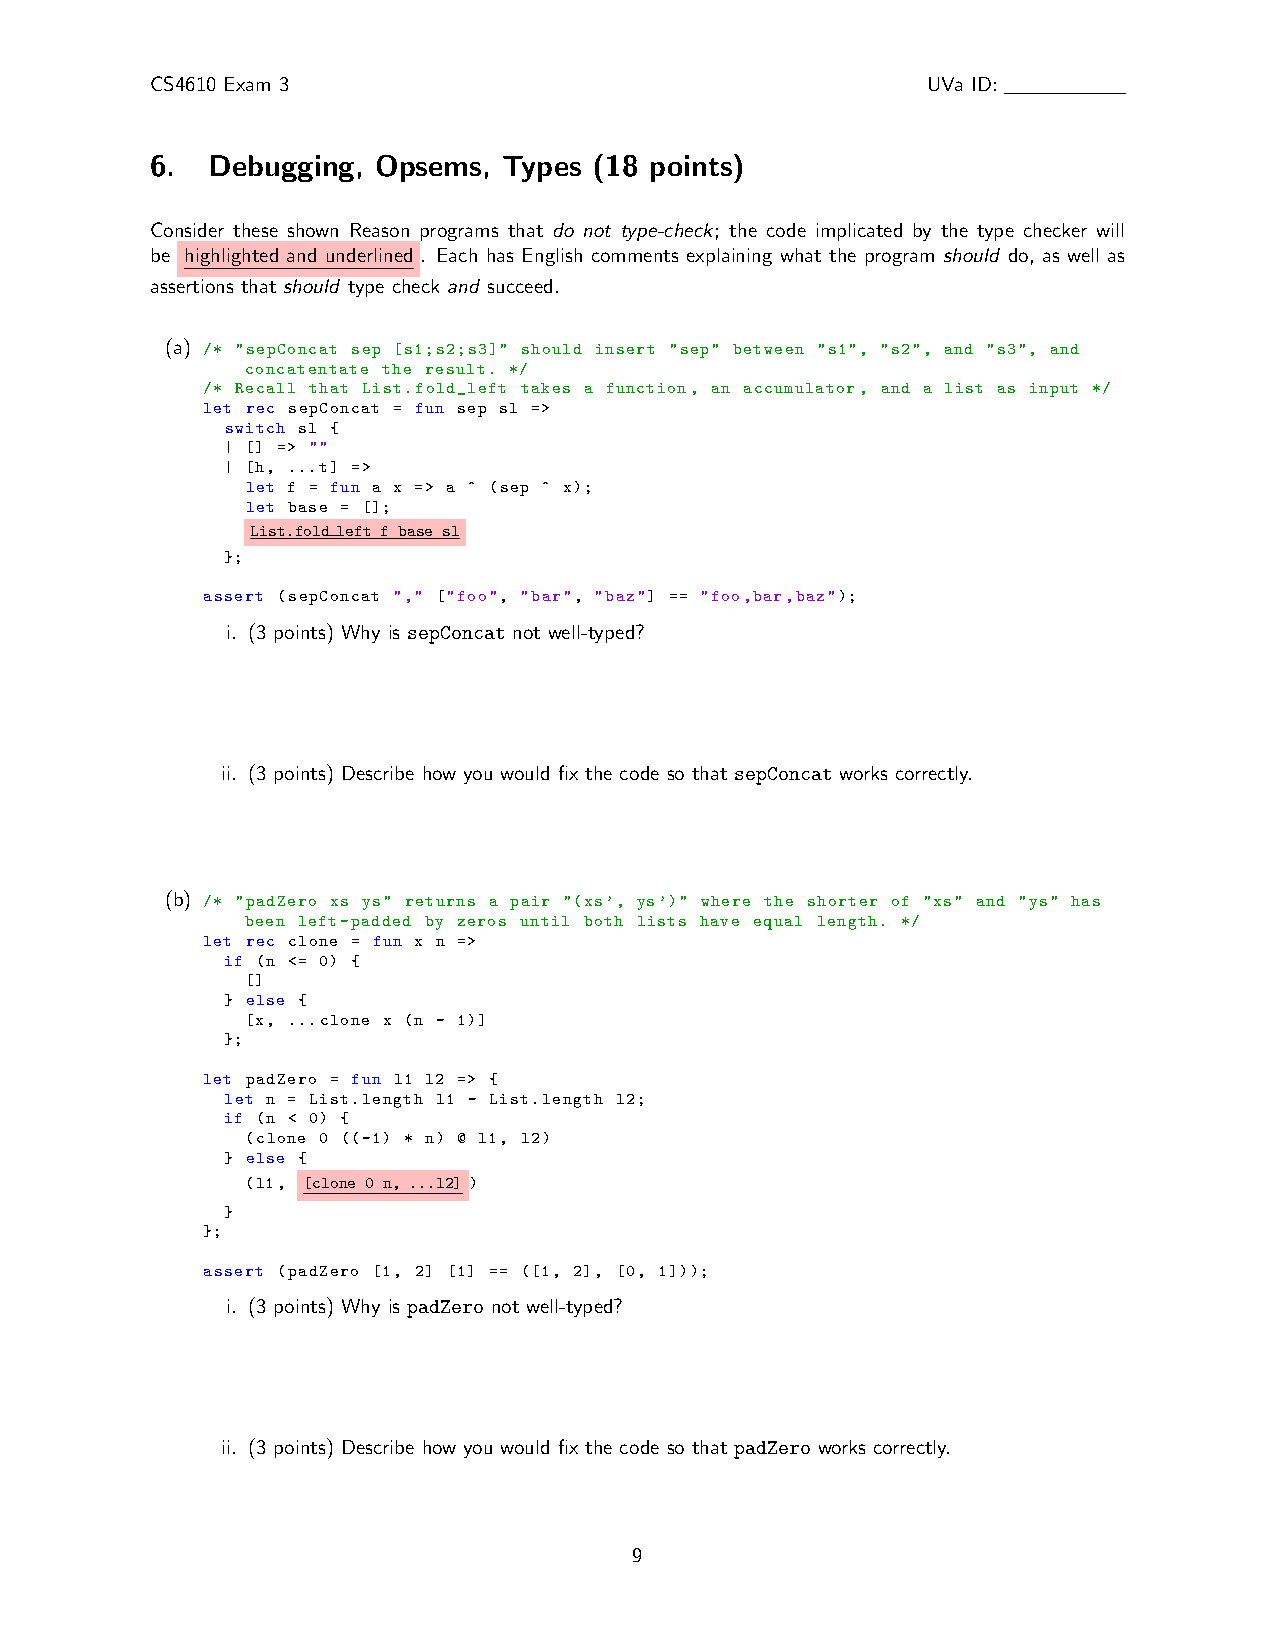
\includegraphics[width=0.98\linewidth,page=1]{study/study_a.pdf}}
\newpage
\noindent\fbox{\includegraphics[width=0.98\linewidth,page=2]{study/study_a.pdf}}
\newpage
\subsection{Version B}
\noindent\fbox{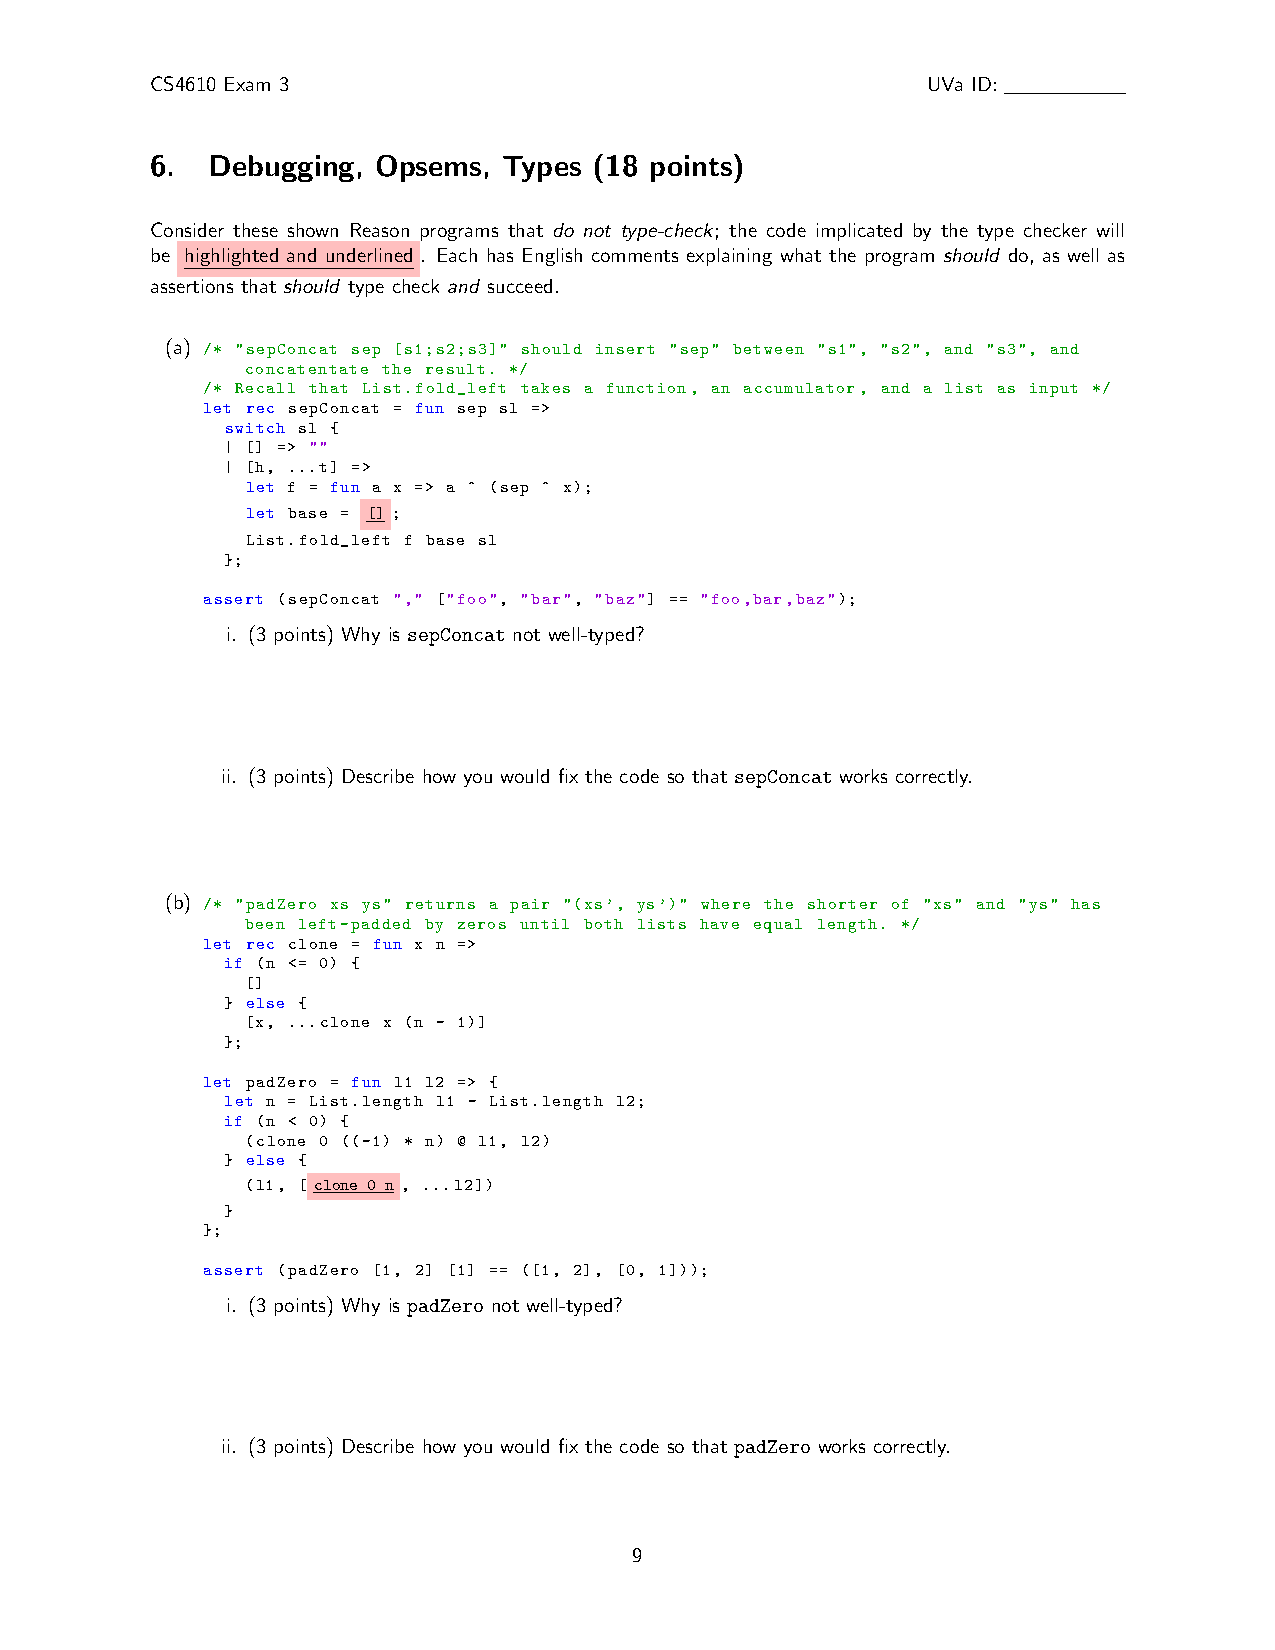
\includegraphics[width=0.98\linewidth,page=1]{study/study_b.pdf}}
\newpage
\noindent\fbox{\includegraphics[width=0.98\linewidth,page=2]{study/study_b.pdf}}


\end{document}
